\documentclass[12pt,a4paper]{article}
\usepackage{graphicx, booktabs, siunitx, amsmath, geometry, float}
\usepackage{subcaption}
\geometry{margin=2.5cm}
\title{M2: Operational Amplifier Basic Circuits}
\author{Gregorio Jaca U8L9B9 gregorio.jaca@gmail.com , \\ Peter Tallosy K14WR1 peter@tallosy.hu }
\date{\today}

\begin{document}
\maketitle

\begin{abstract}
In this laboratory excercise we investogated the characteristics and applications of operational amplifiers (op-amps). We constructed and analyzed five fundamental op-amp circuits: an inverting amplifier, an adder, a voltage follower, a differentiator, and an integrator. The behavior of these circuits was examined using various input signals, and the experimental results were compared with theoretical predictions. We characterized properties such as gain, saturation, frequency response, and the transformative effects of these circuits on different waveforms.
\end{abstract}

\section{Measurement Instruments}
The following equipment was used for the measurements:
\begin{itemize}
    \item DC Power Supply: Siglent SPD3303C
    \item Digital Multimeter: Siglent SDM 3045X and UNI-T UT334+
    \item Function Generator: RIGOL DG811 SiFi II 20MHz AWG
    \item Oscilloscope: SIGLENT SDS 1072CML Digital Oscilloscope
    \item Op-Amps: UA741CN, TL071CP
    \item Resistors and Capacitors of various values.
\end{itemize}

\section{Results and Discussion}

\subsection{M1: Inverting Amplifier}
We constructed an inverting amplifier using a UA741CN op-amp. The circuit was configured with a feedback resistor \(R_v = \SI{470}{\kilo\ohm}\) and an input resistor \(R_s = \SI{100}{\kilo\ohm}\). The theoretical voltage gain (\(A_{th}\)) of this configuration is given by:
\begin{equation}
    A_{th} = -\frac{R_v}{R_s} = -\frac{\SI{470}{\kilo\ohm}}{\SI{100}{\kilo\ohm}} = -4.7
\end{equation}
The input DC voltage was varied in \SI{100}{\milli\volt} increments, and the output voltage was measured. The measured data is plotted in Figure \ref{fig:inverting_amp_gain}.

\begin{figure}[H]
    \centering
    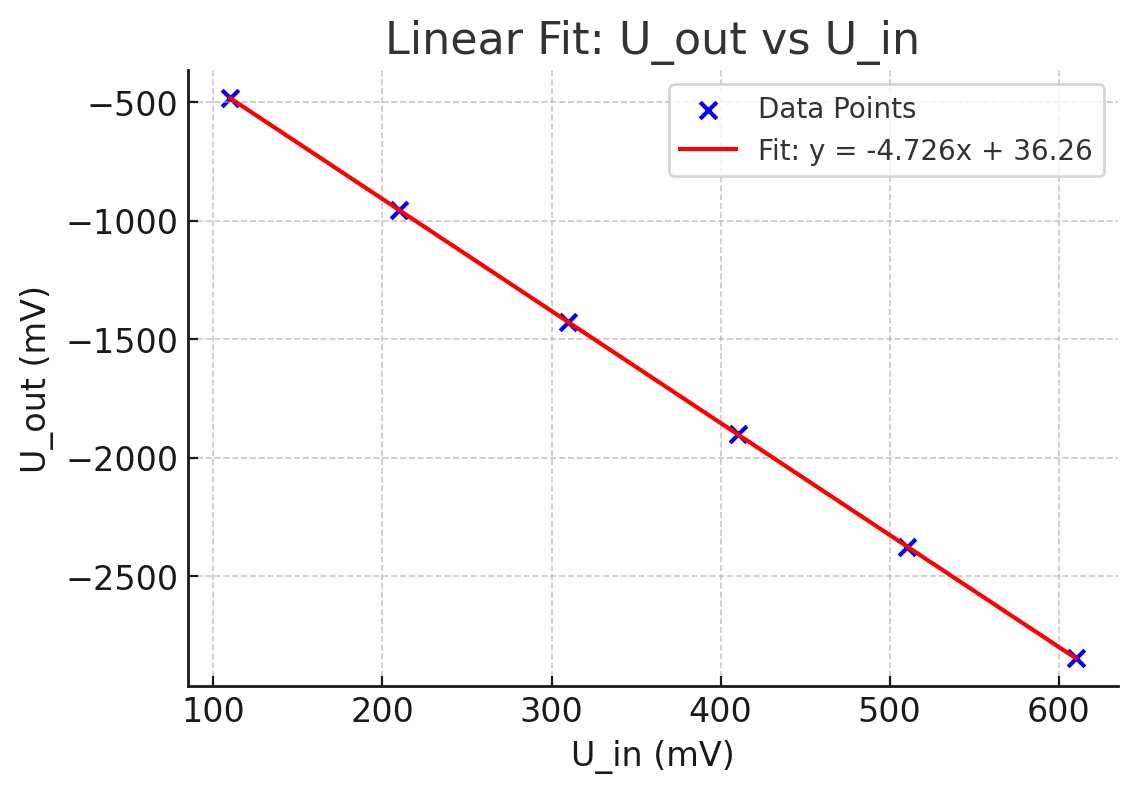
\includegraphics[width=0.6\linewidth]{inverter_fit.png} % 
    \caption{Measured output voltage as a function of input voltage for the inverting amplifier. The red line represents a linear fit to the non-saturated region.}
    \label{fig:inverting_amp_gain}
\end{figure}

From the linear region of the measured data (up to \(U_{in} = \SI{600}{\milli\volt}\)), the experimental gain (\(A_{exp}\)) was determined from the slope of a linear fit, which was found to be \(A_{exp} = -4.723\). This value is in excellent agreement with the theoretical gain, with a relative difference of approximately 0.55. Beyond an input of \SI{600}{\milli\volt}, the output voltage saturated at approximately \(U_{sat} = \SI{-3.13}{\volt}\), which is consistent (but smaller than we expected) with the limits imposed by the \(\pm\SI{5}{\volt}\) supply voltage.

\begin{figure}[H]
    \centering
    \includegraphics[width=0.6\linewidth]{inverter_saturator.png} % 
    \caption{Measured output voltage as a function of input voltage for the inverting amplifier including the saturation region}
    \label{fig:inverting_amp_saturated}
\end{figure}

\subsection{M2: Adder Circuit}
An adder circuit was built with \(R_1 = R_2 = R_s = R_v = \SI{1}{\kilo\ohm}\). The theoretical output is the negative sum of the inputs: \(U_{out} = -(U_{in1} + U_{in2})\). We tied the inputs together (\(U_{in1} = U_{in2} = U_{in}\)), which implies that \(U_{out} = -2(U_{in})\), and the Amplification will be \(A = U_{out}/U_{in} = -2\). The fit in Fig. \ref{fig:adder} shows a slope of -2, experimentally confirming our prediction and proving the additive property of the circuit.

\begin{figure}[H]
    \centering
    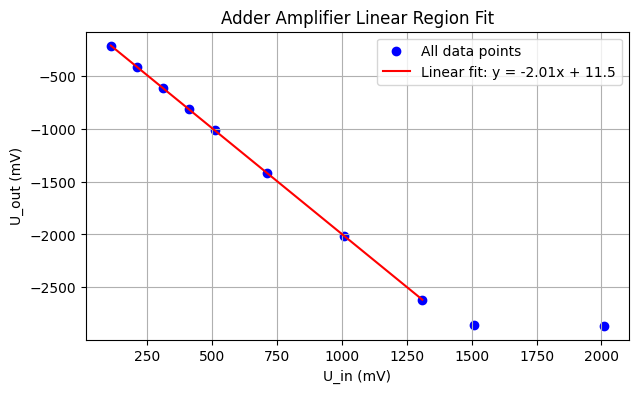
\includegraphics[width=0.6\linewidth]{adder_fit.png} % 
    \caption{Measured output voltage as a function of input voltage for the adder amplifier including the saturation region}
    \label{fig:adder}
\end{figure}

\subsection{M3: Voltage Follower}
A voltage follower, or buffer amplifier, was constructed using a TL071CP op-amp. This circuit has a theoretical gain of +1. We applied a \SI{1}{\kilo\hertz}, \SI{100}{\milli\volt} peak-to-peak sinusoidal signal to the input. At low frequencies, the output signal was an exact replica of the input, demonstrating the unity gain characteristic of the follower, as seen in Figure \ref{fig:follower_unity}.

\begin{figure}[H]
    \centering
    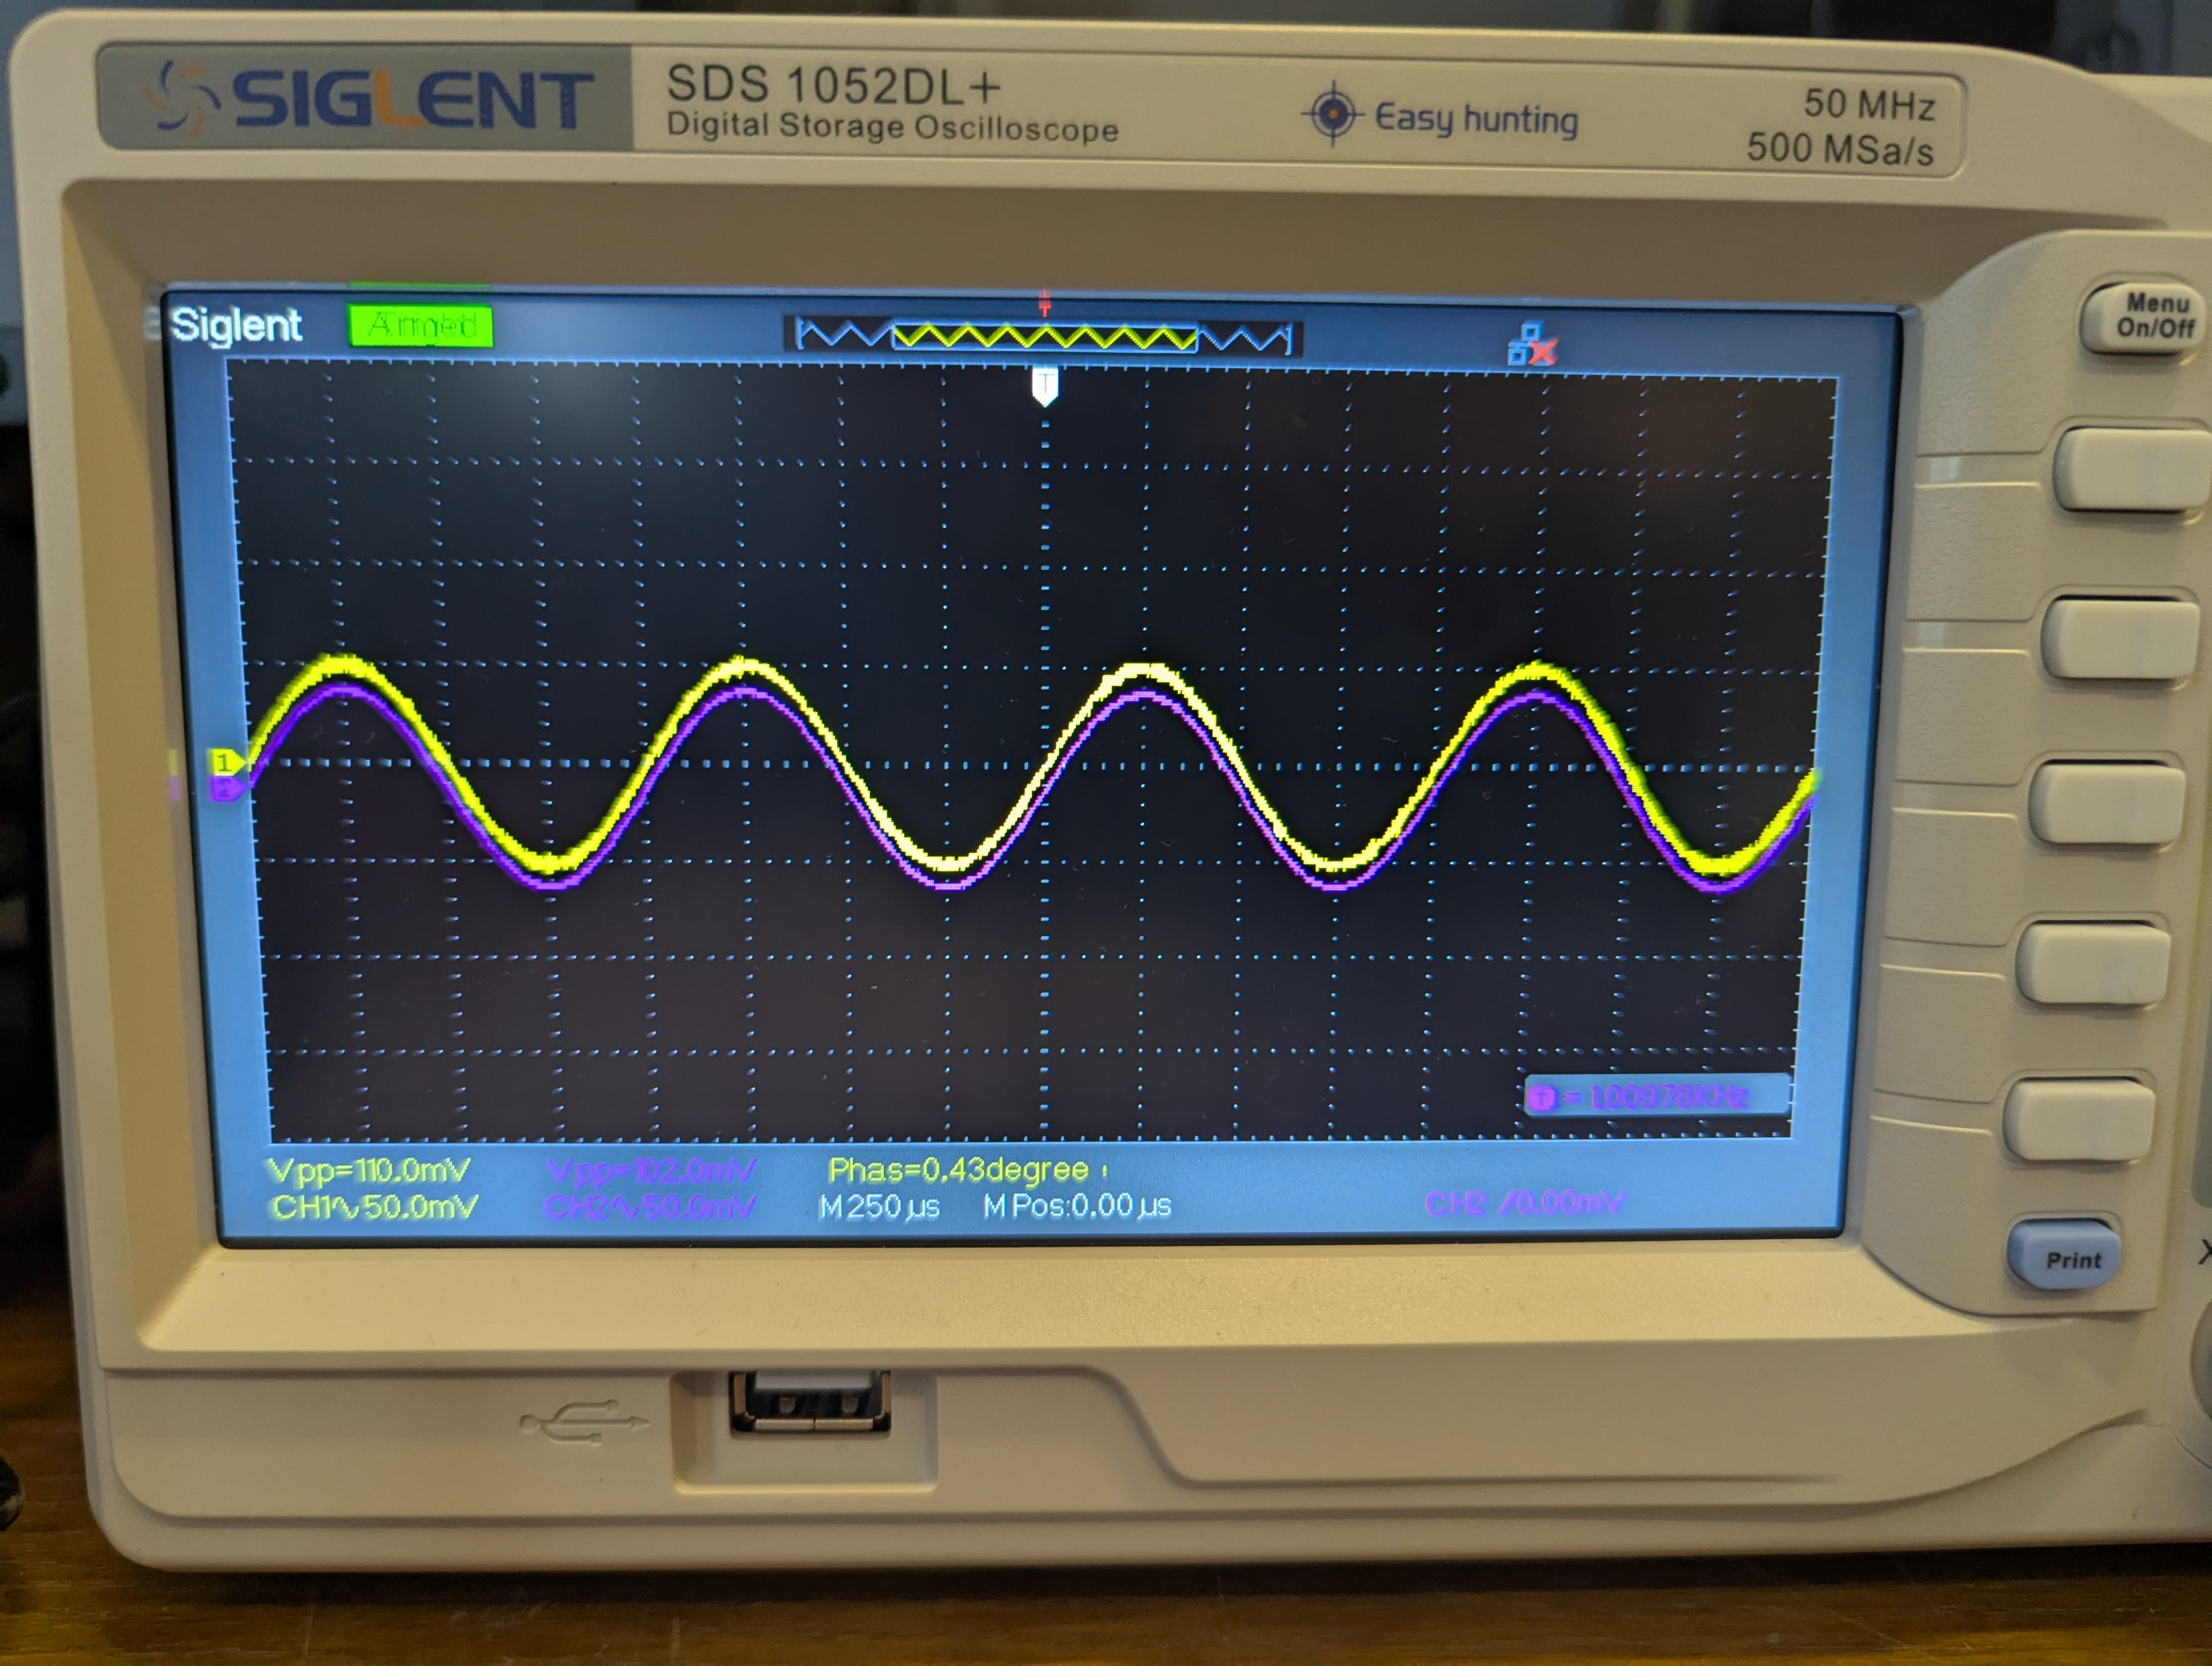
\includegraphics[width=0.6\linewidth]{voltage_follower.jpg} 
    \caption{Input (purple) and output (yellow) signals of the voltage follower, showing the output closely tracking the input, confirming a gain of approximately +1.}
    \label{fig:follower_unity}
\end{figure}

As the frequency was increased, a phase difference became apparent, and the output amplitude started to decrease. The upper cutoff frequency, \(f_c\), is the frequency at which the output voltage amplitude drops to \(1/\sqrt{2}\) of its low-frequency value.
%LLM-UNCERTAIN: The measured value for the cutoff frequency fc is missing. Please add the value.


\subsection{M4: Differentiator}
A differentiator circuit was built with \(C = \SI{10}{\nano\farad}\) and \(R_v = \SI{100}{\kilo\ohm}\). The circuit\'s output is proportional to the time derivative of the input signal. We tested the circuit with sine, square, and triangle wave inputs. Figure \ref{fig:differentiator_no} shows the output waveforms, which are noisy and there is ringing, especially at the points where the derivative is discontinuous, especially for the triangle and square wave inputs. 

To improve stability, a small capacitor (\(C_p = \SI{100}{\pico\farad}\)) was placed in parallel with the feedback resistor. This capacitor forms a low-pass filter, reducing high-frequency noise. Figure \ref{fig:differentiator} shows the output waveforms with \(C_p\) included. The outputs are visibly smoother and more stable, demonstrating the effectiveness of this technique. As expected, a sine wave input produced a cosine wave, a triangle wave produced a square wave, and a square wave produced sharp spikes.

\begin{figure}[H]
    \centering
    \begin{subfigure}[b]{0.32\linewidth}
        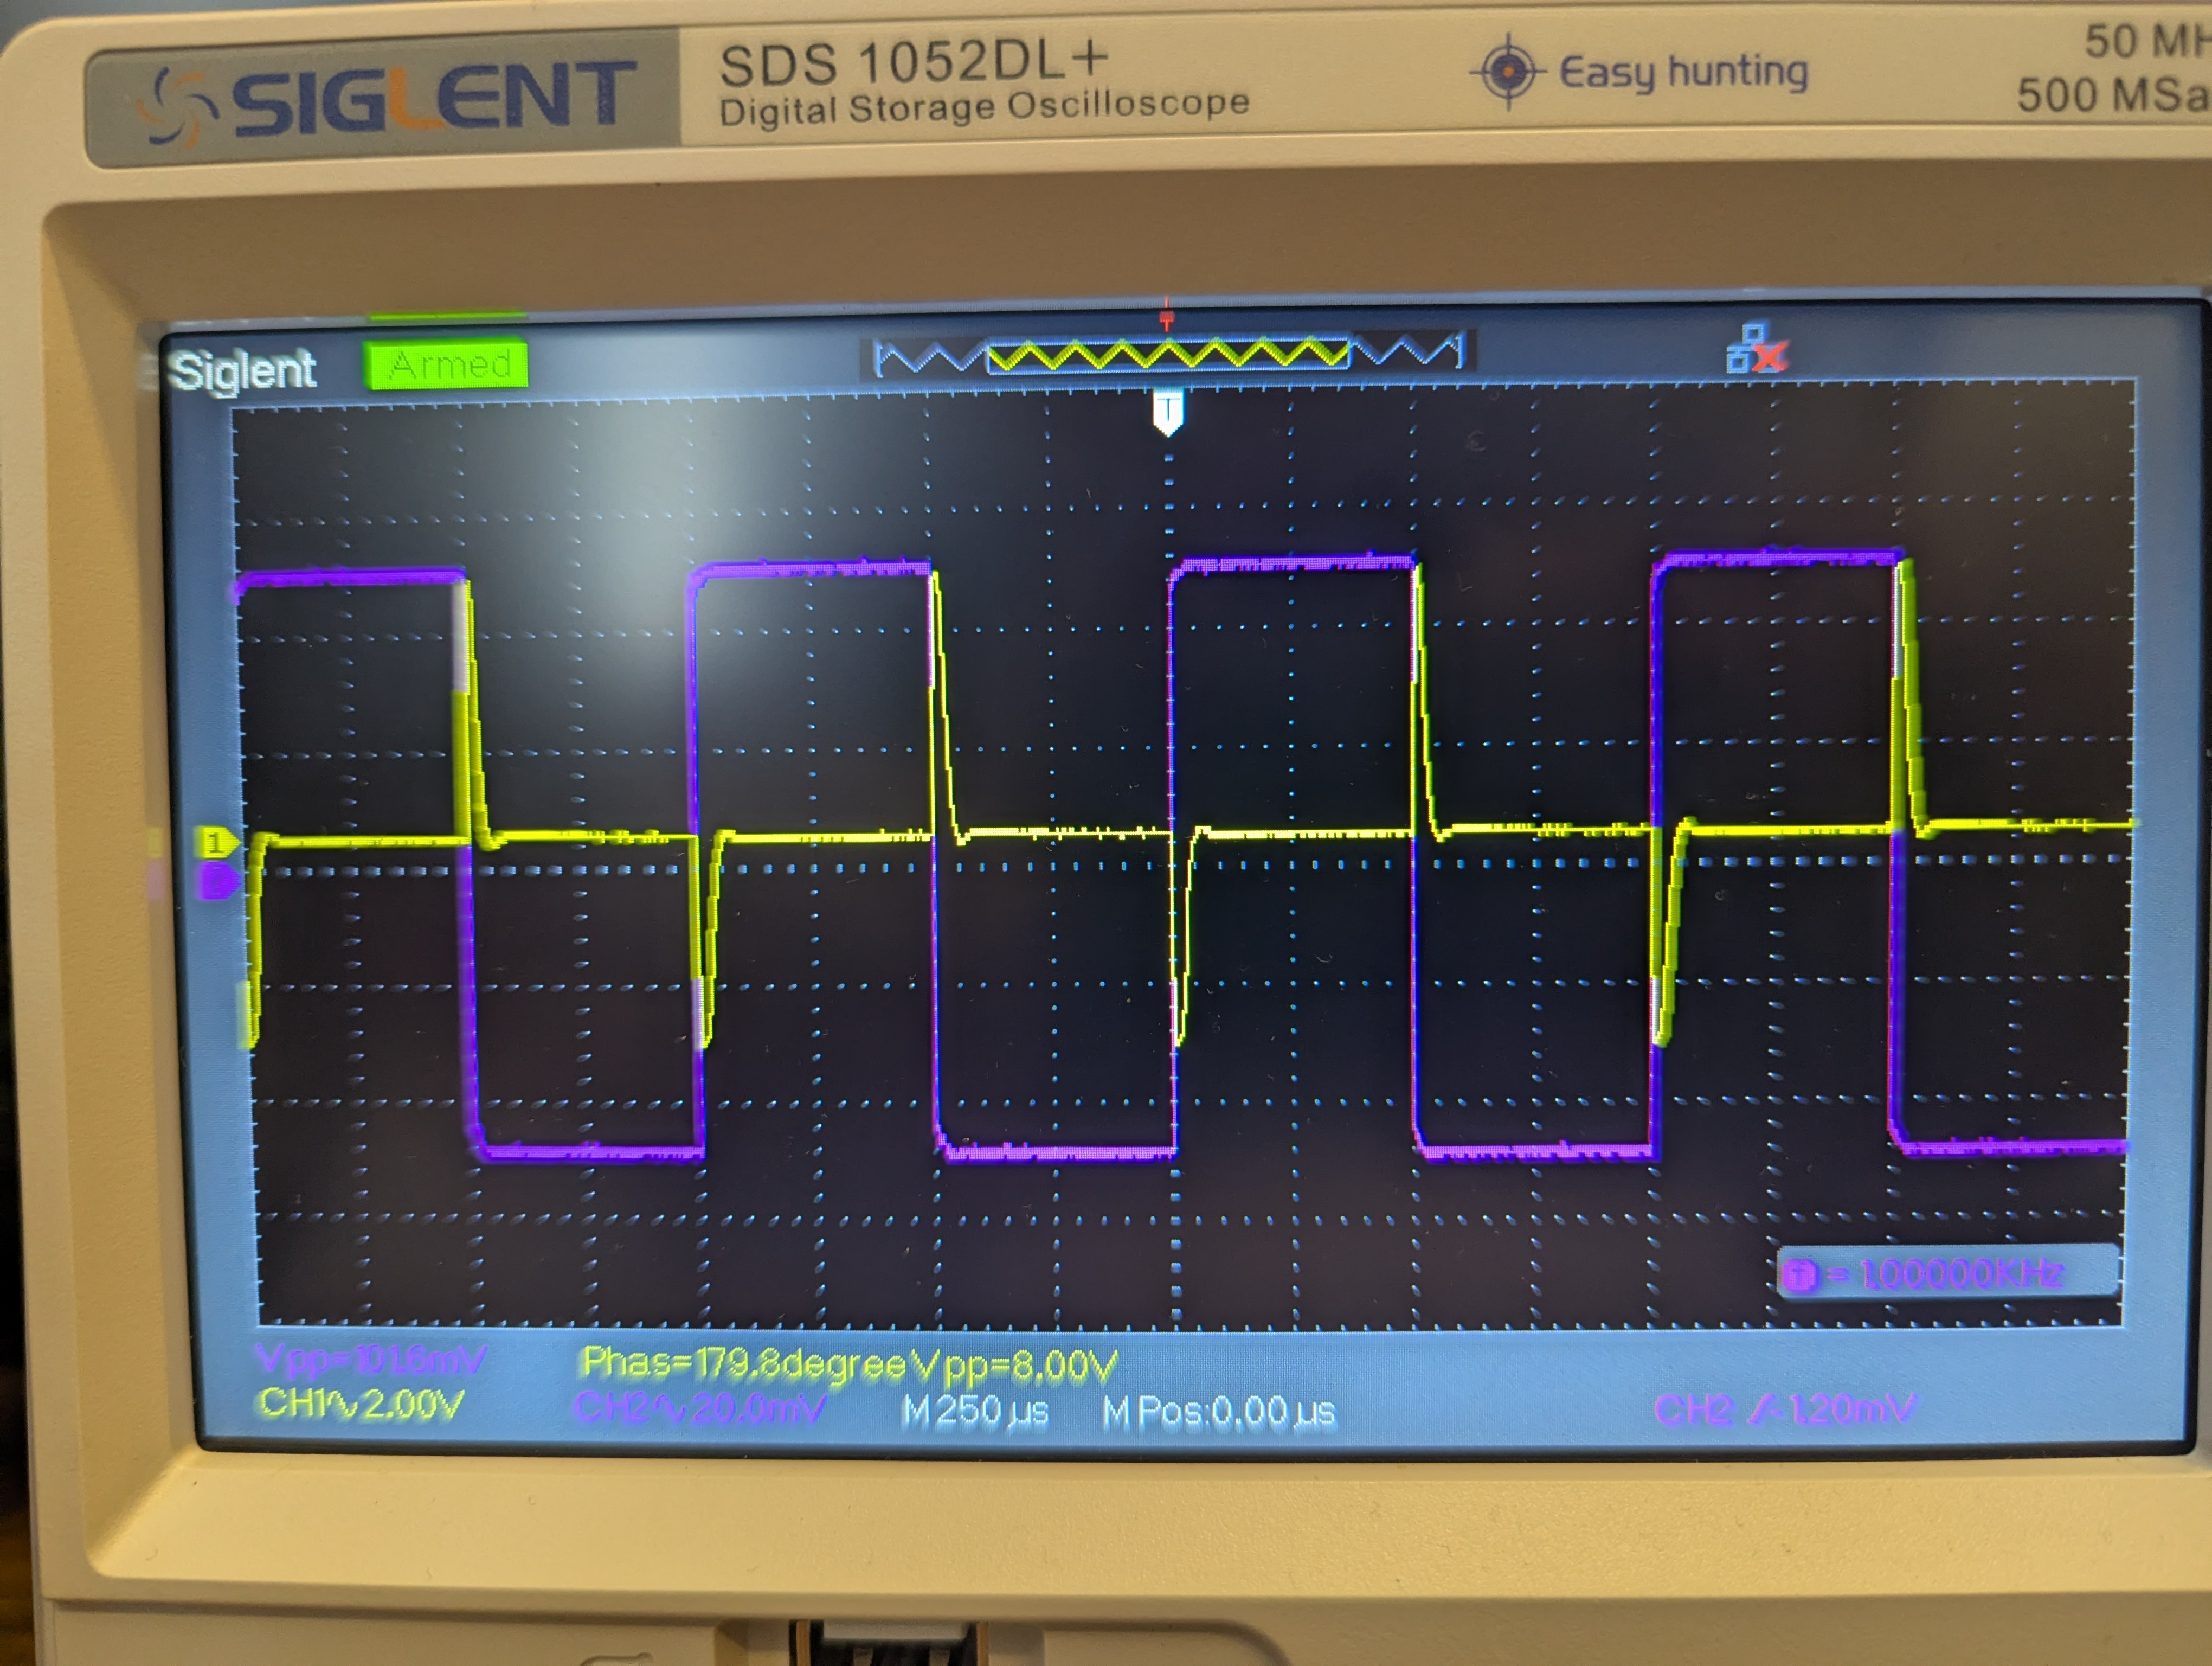
\includegraphics[width=\linewidth]{diff_square.jpg} 
    \end{subfigure}
    \begin{subfigure}[b]{0.32\linewidth}
        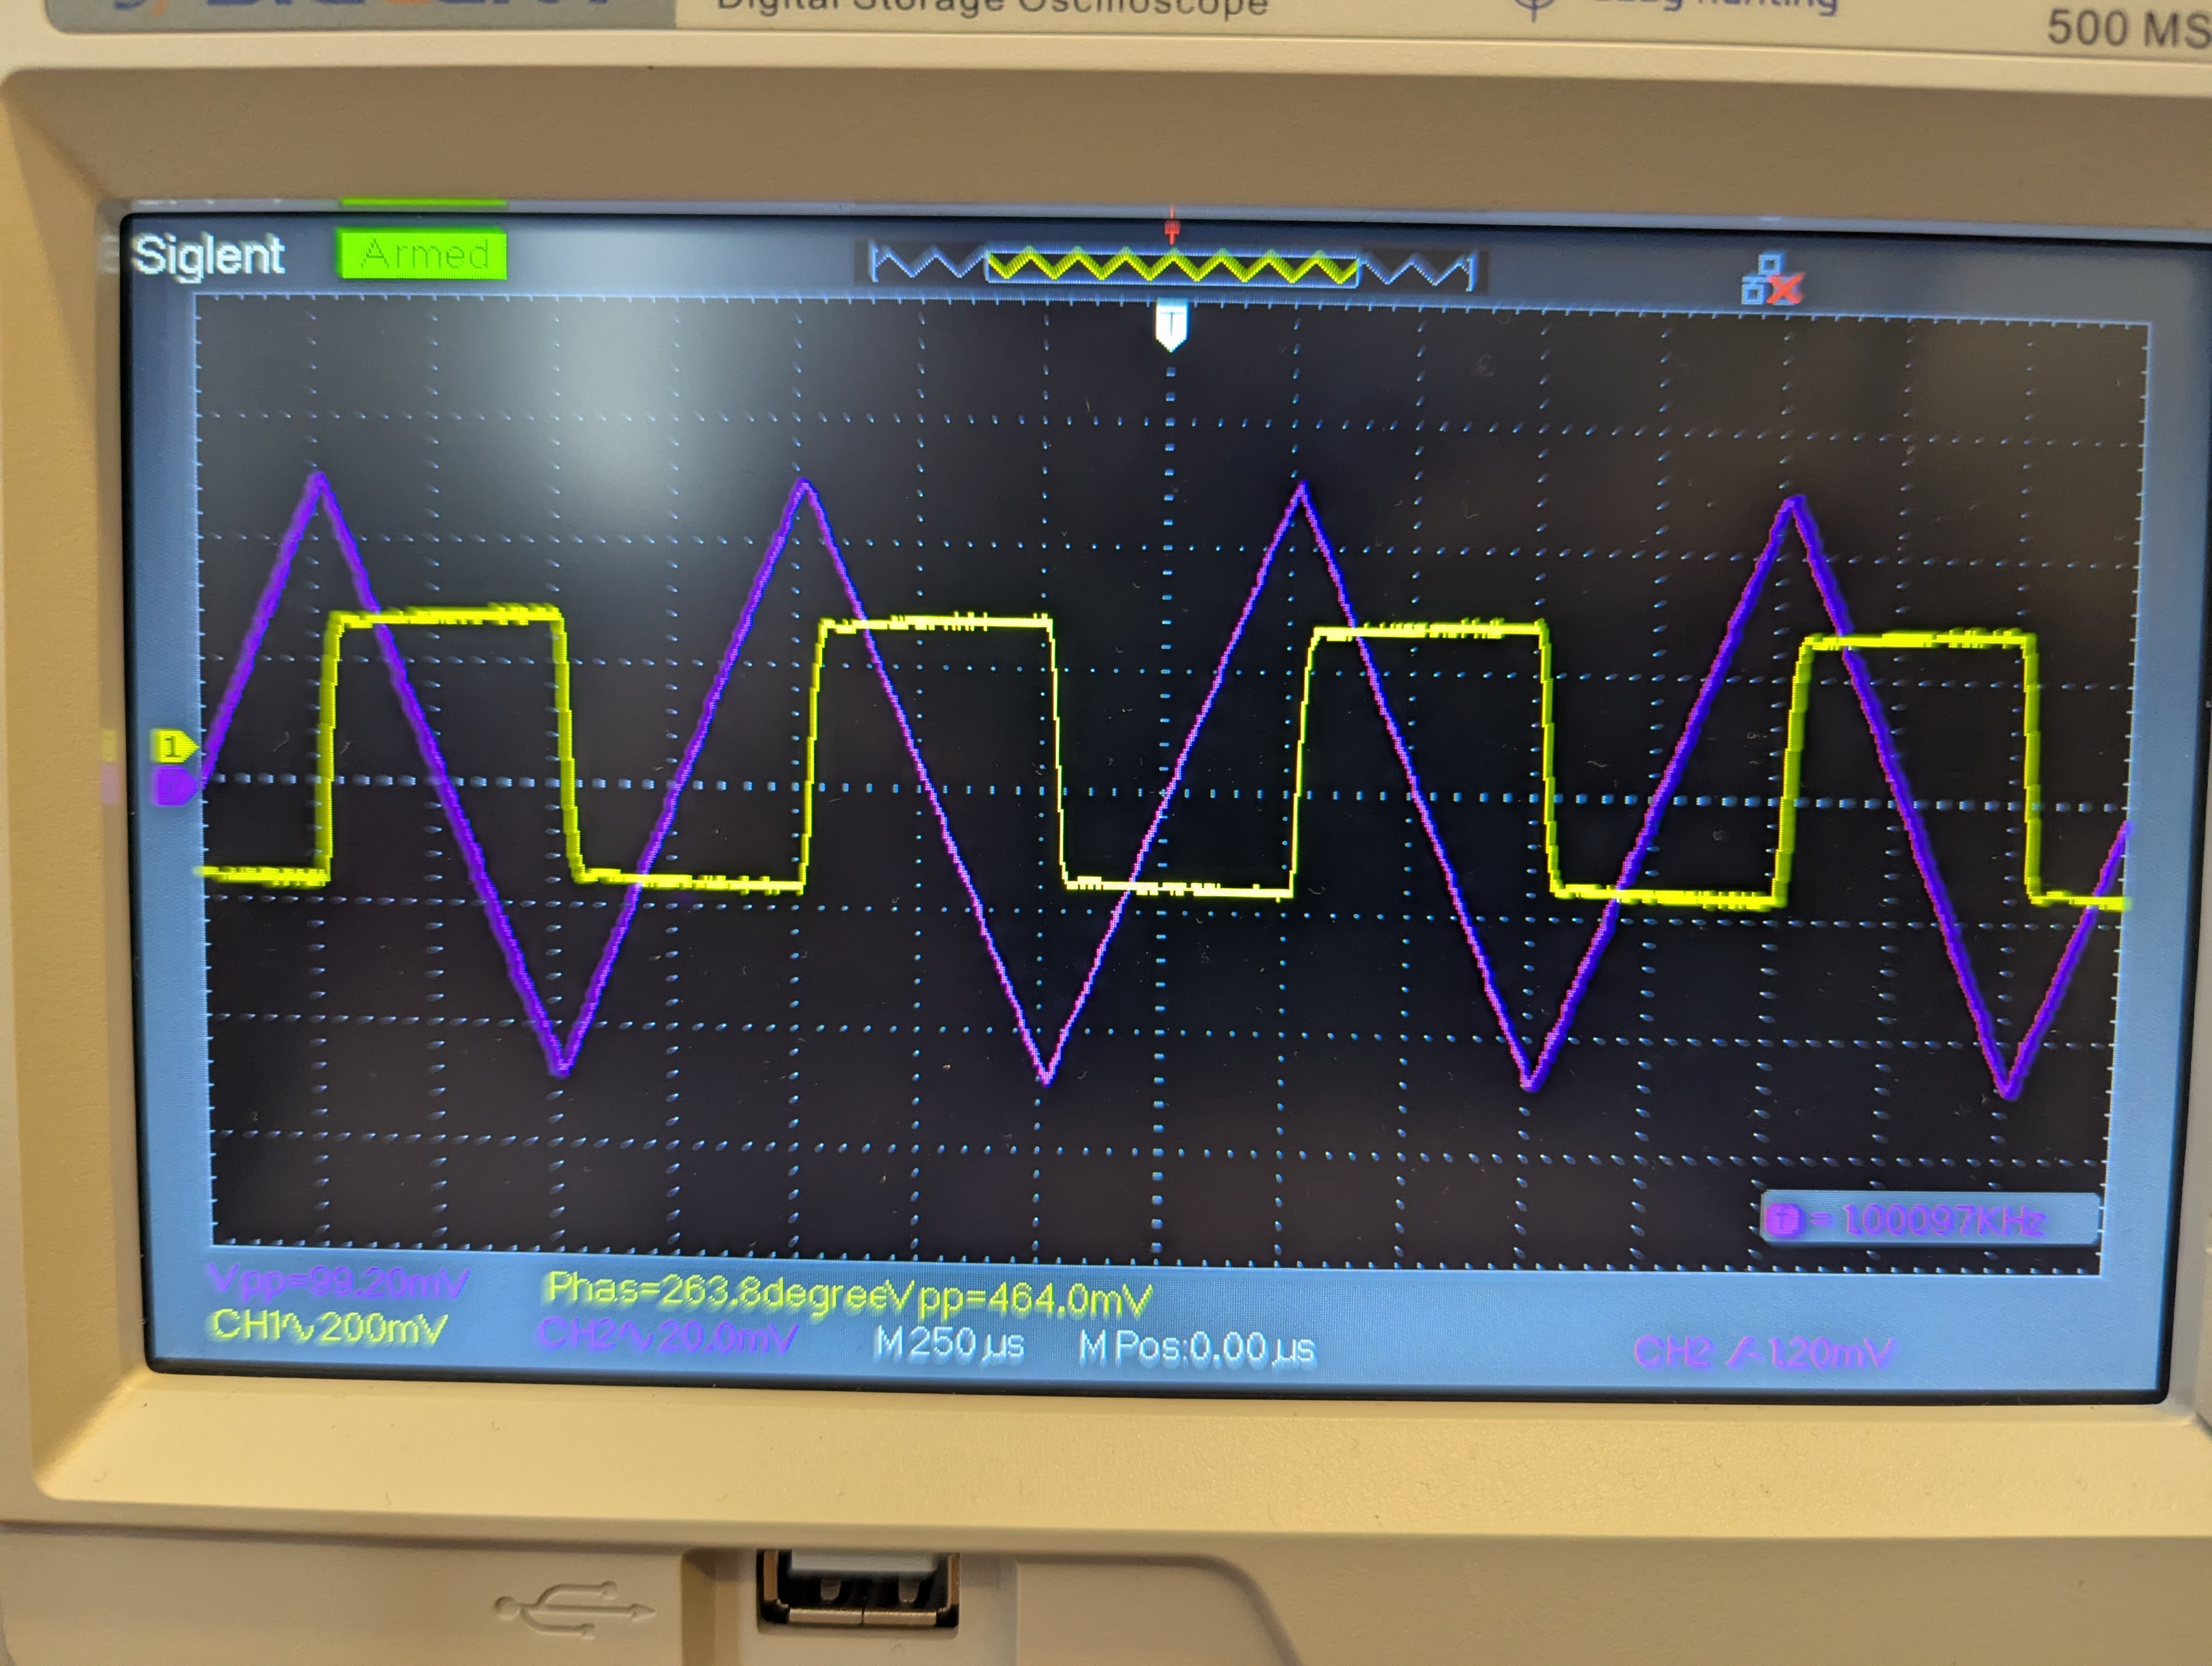
\includegraphics[width=\linewidth]{diff_triangle.jpg} 
    \end{subfigure}
    \caption{Differentiator output waveforms for square and triangle inputs \textbf{with} the stabilizing capacitor \(C_p\).}
    \label{fig:differentiator}
\end{figure}

\begin{figure}[H]
    \centering
    \begin{subfigure}[b]{0.32\linewidth}
        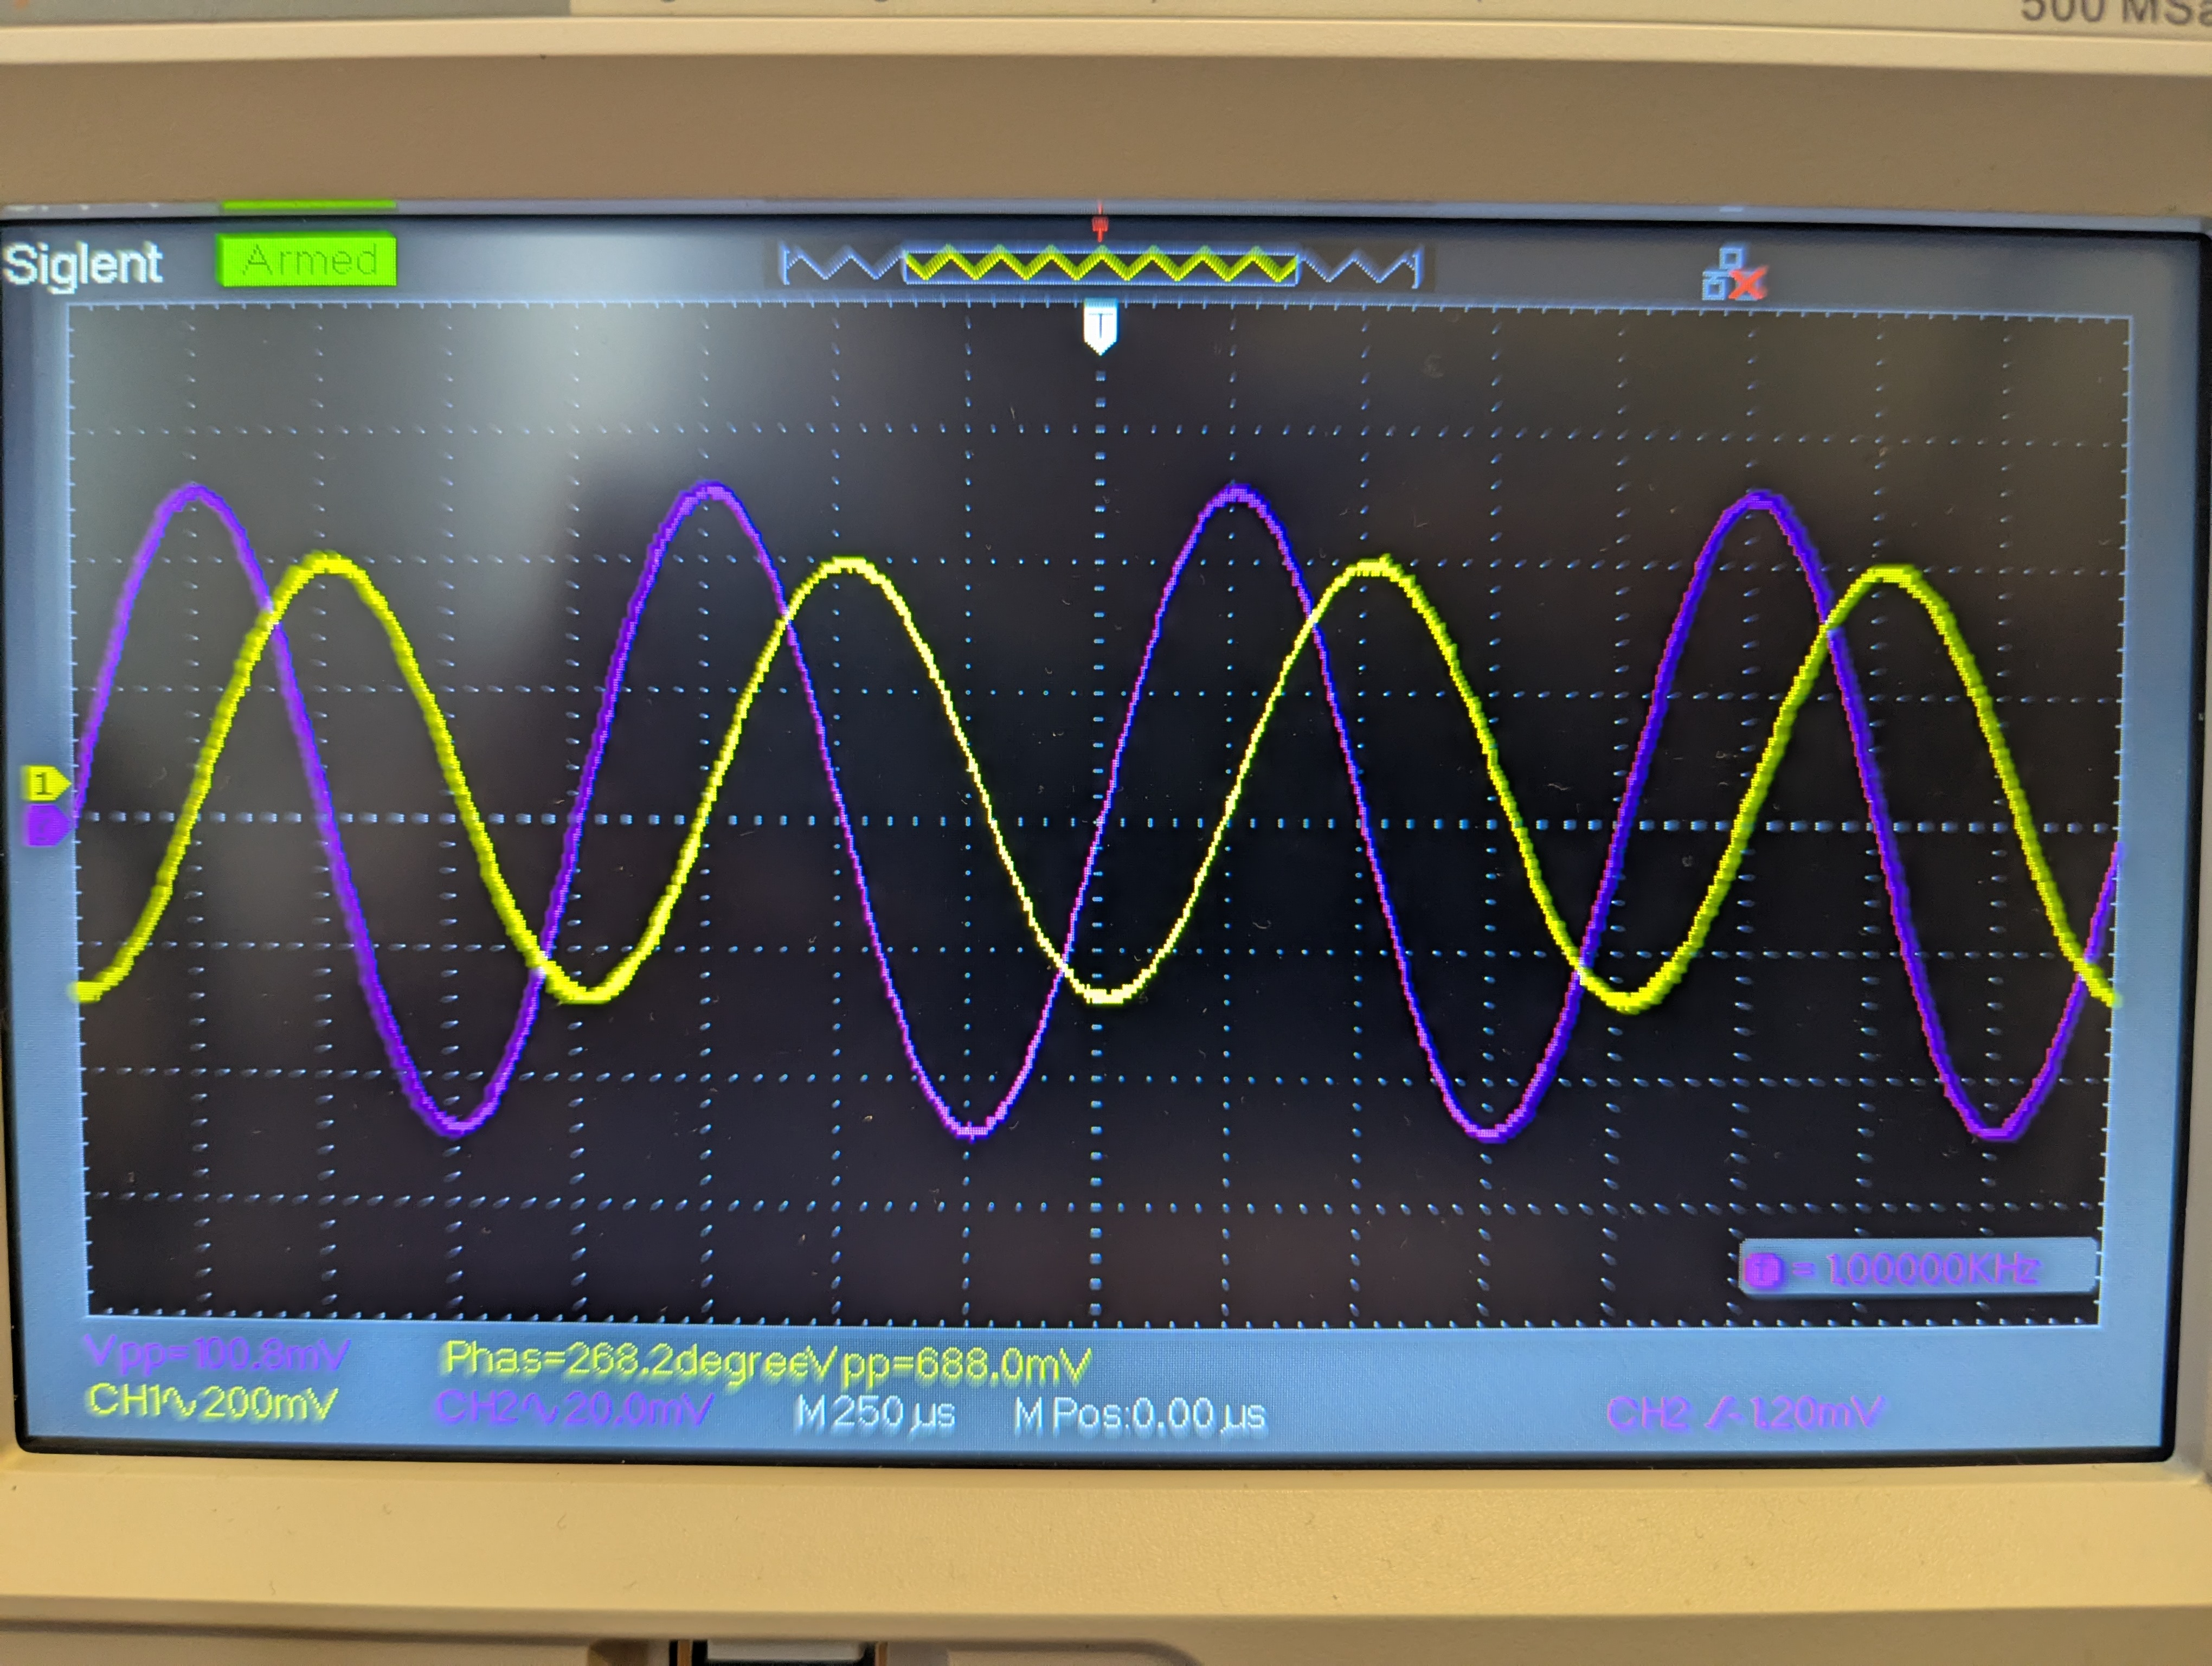
\includegraphics[width=\linewidth]{diff_sine_no.jpg} 
    \end{subfigure}
    \begin{subfigure}[b]{0.32\linewidth}
        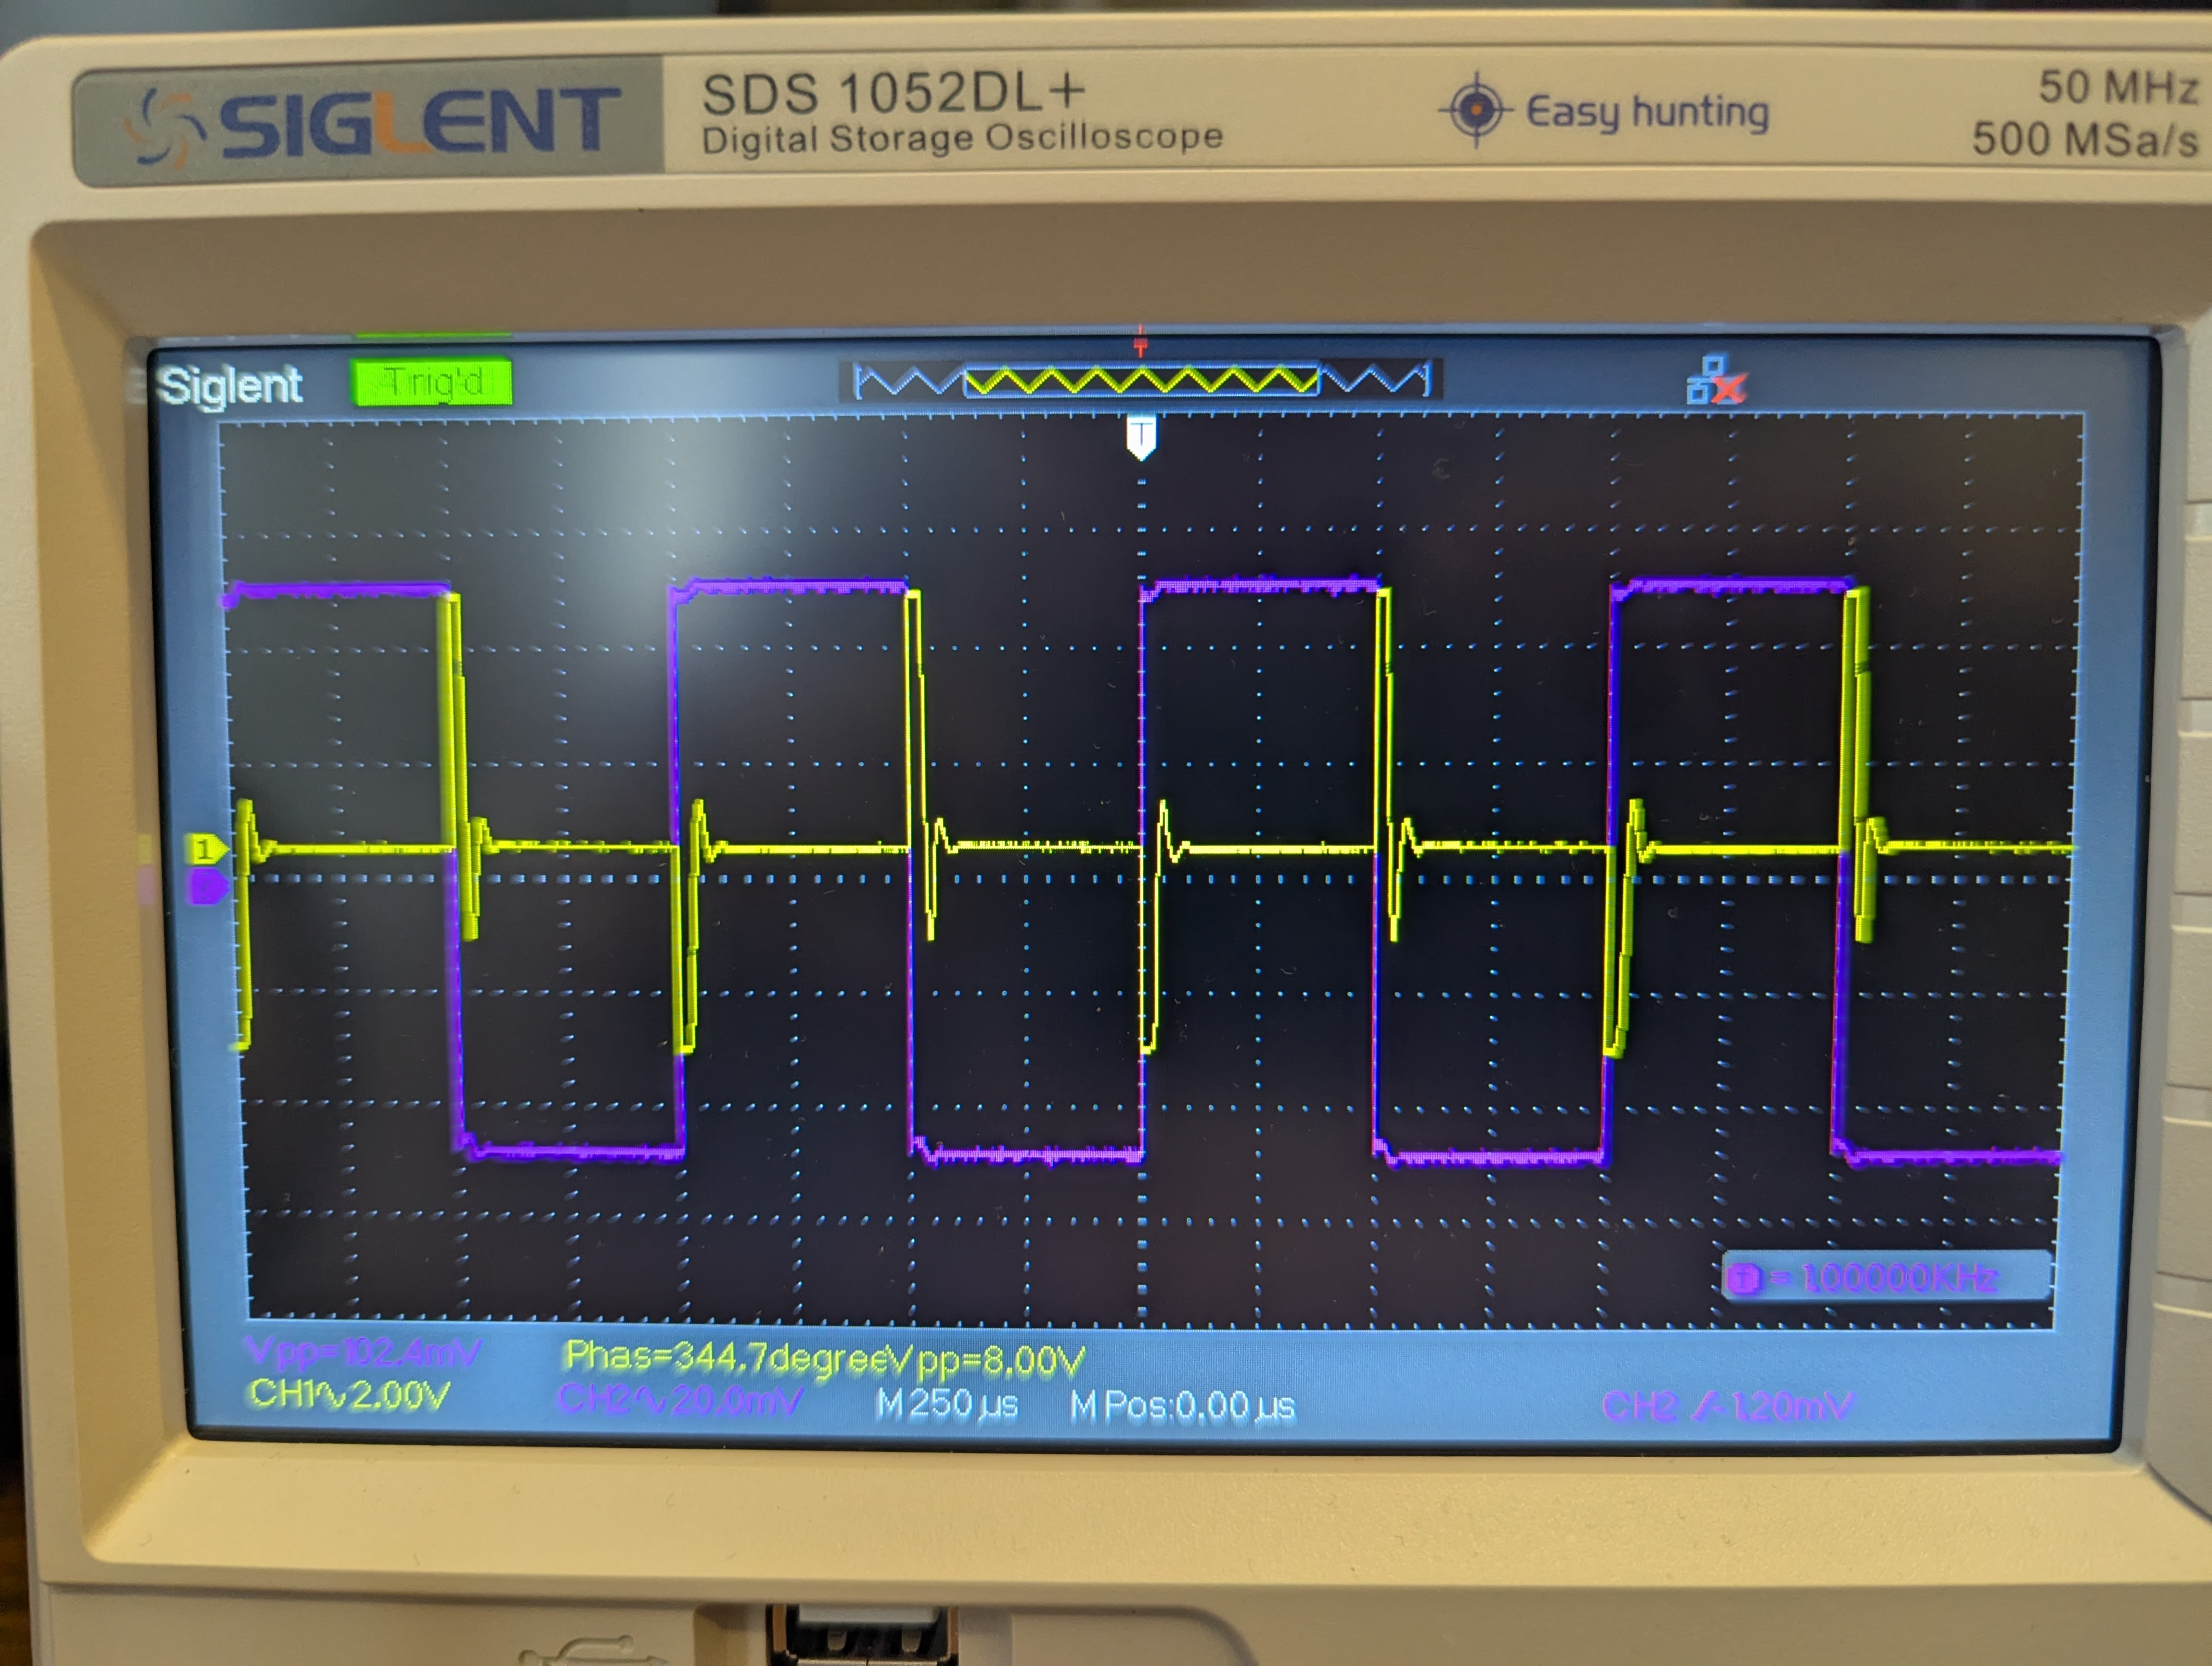
\includegraphics[width=\linewidth]{diff_square_no.jpg} 
    \end{subfigure}
    \begin{subfigure}[b]{0.32\linewidth}
        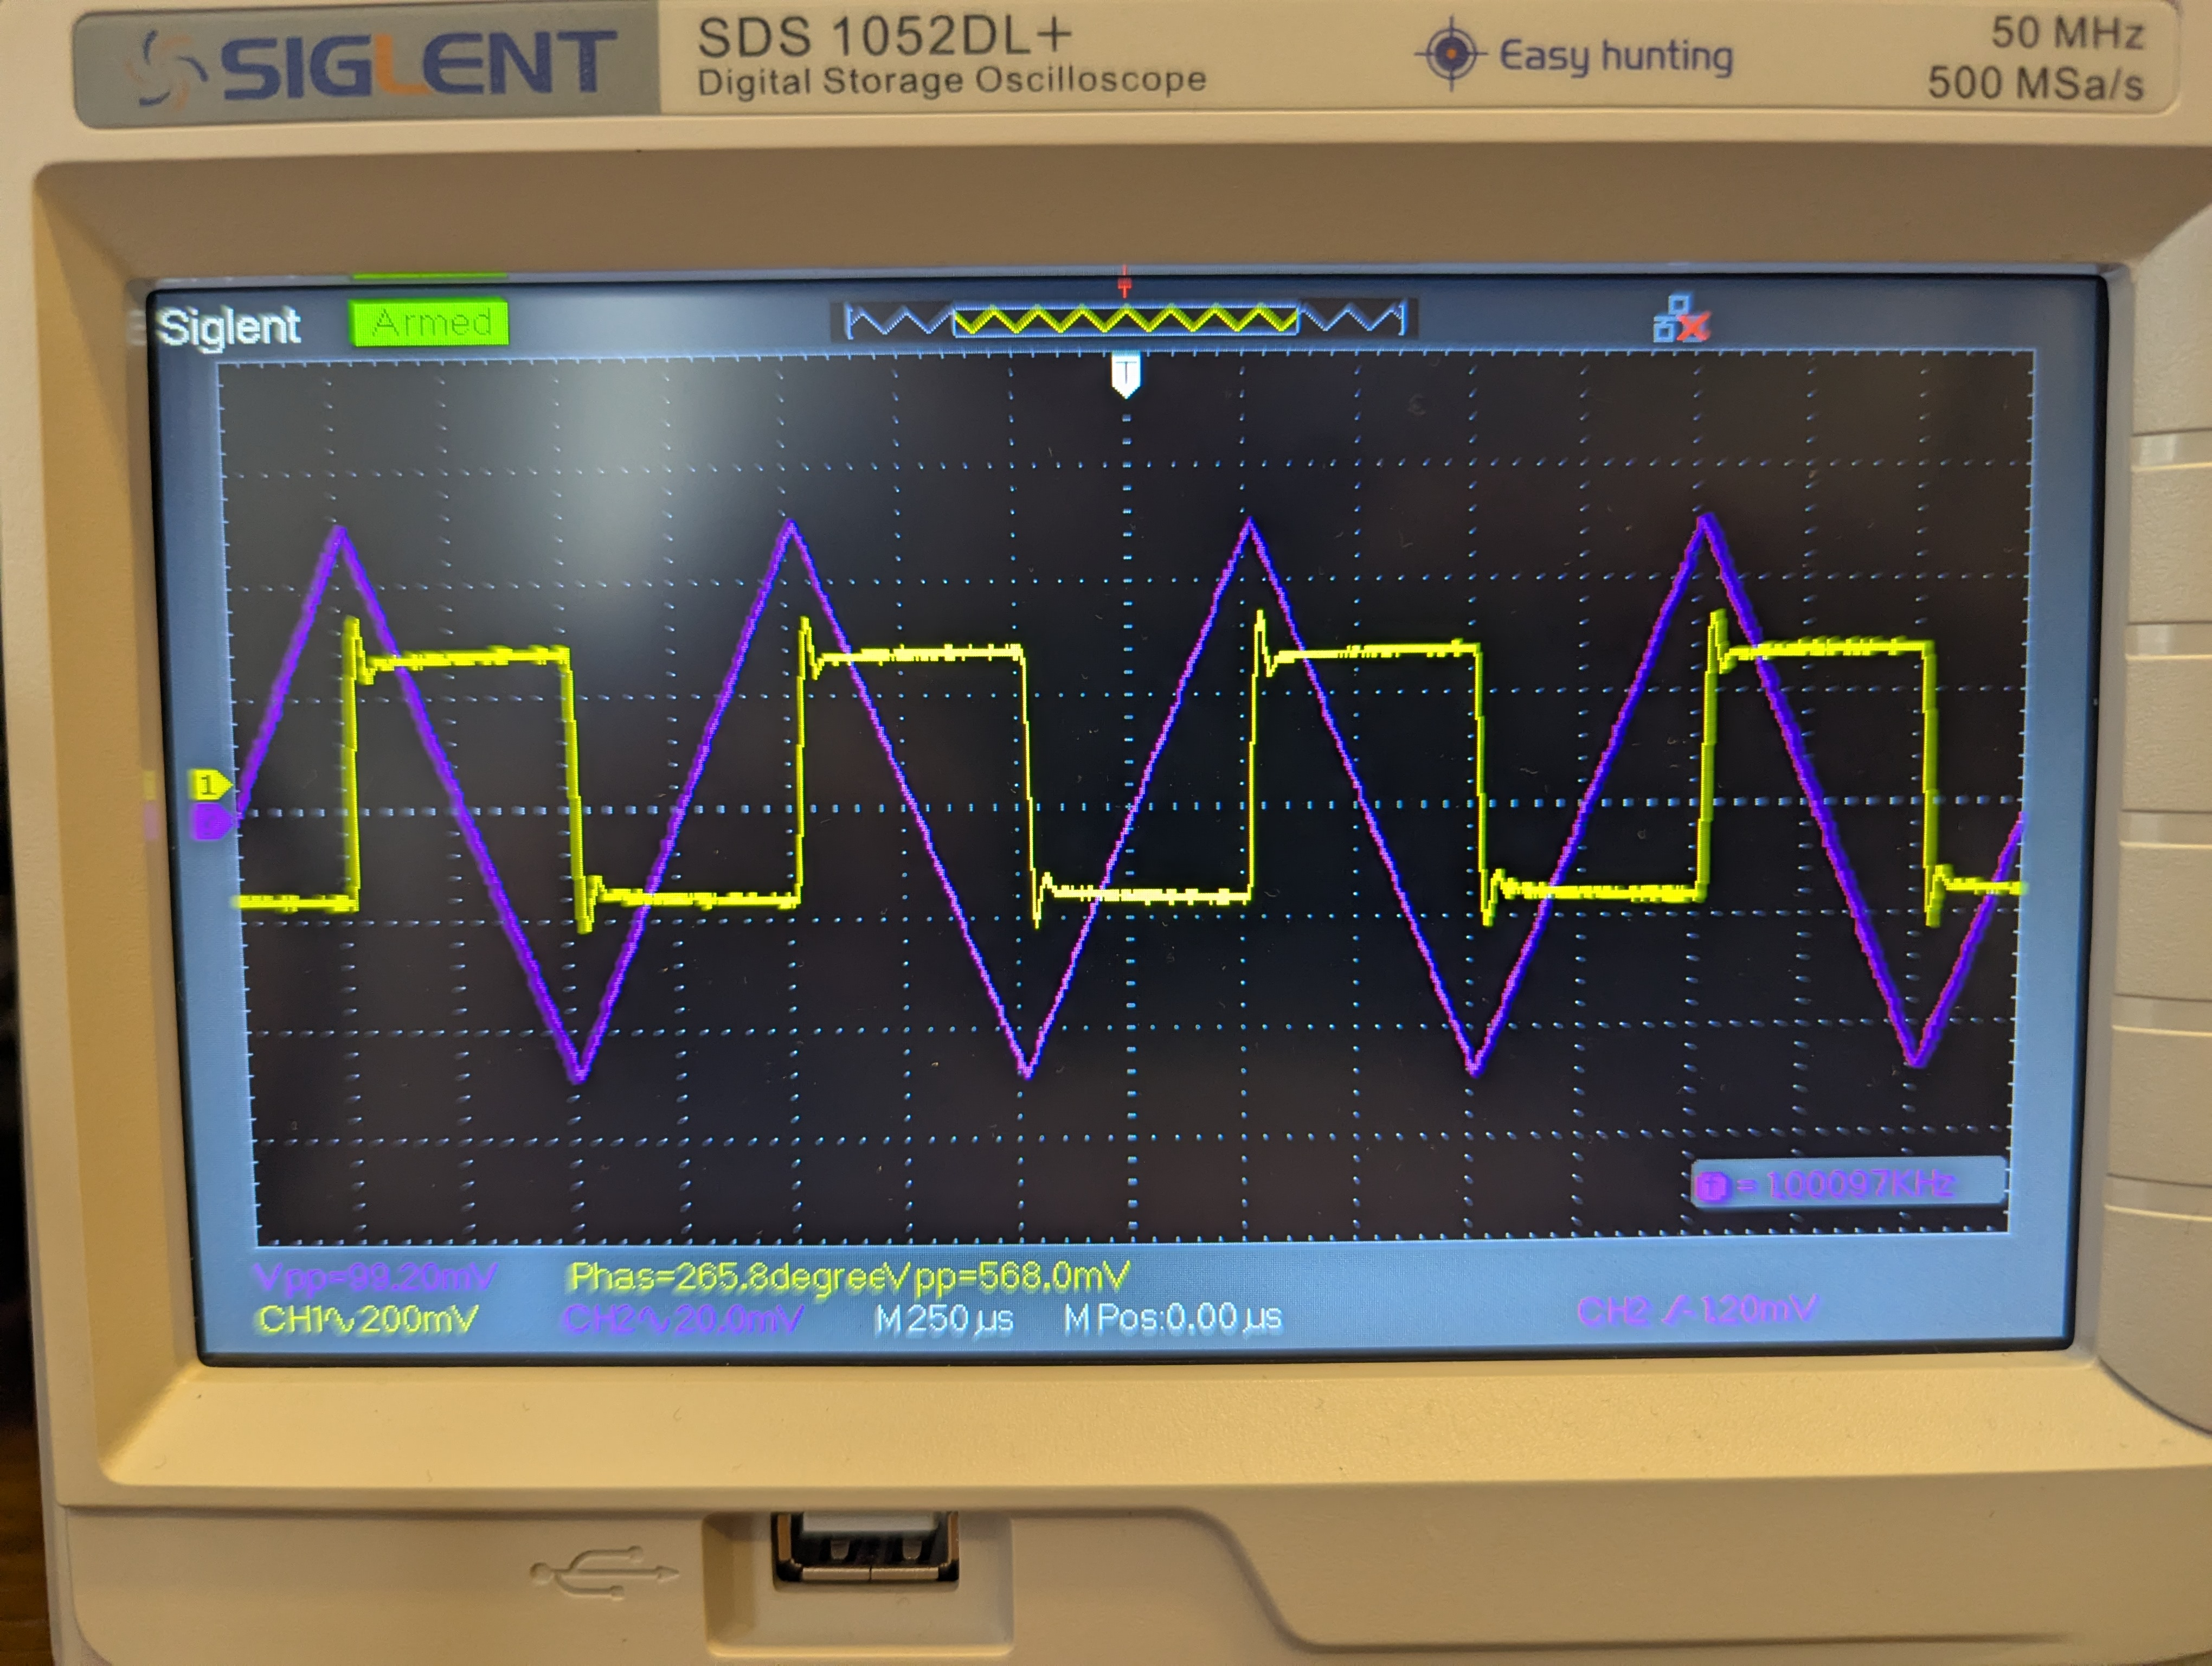
\includegraphics[width=\linewidth]{diff_triangle_no.jpg} 
    \end{subfigure}
    \caption{Differentiator output waveforms for sine, square, and triangle inputs \textbf{without} the stabilizing capacitor \(C_p\).}
    \label{fig:differentiator_no}
\end{figure}


\subsection{M5: Integrator}
The integrator circuit was constructed with \(C = \SI{10}{\nano\farad}\) and \(R_s = \SI{100}{\kilo\ohm}\). The output is proportional to the time integral of the input. Without a feedback resistor, small DC offsets at the input can cause the integrator\'s output to drift and eventually saturate, as shown in Figure \ref{fig:integrator_no}.

To counteract this, a large resistor (\(R_p = \SI{10}{\mega\ohm}\)) was placed in parallel with the capacitor. This resistor provides DC feedback, preventing saturation and ensuring stable operation. Figure \ref{fig:integrator_} shows the stable, integrated waveforms. As predicted, a square wave input produced a triangle wave, a sine wave produced a negative cosine wave, and a triangle wave produced a series of parabolas.

\begin{figure}[H]
    \centering
    \begin{subfigure}[b]{0.32\linewidth}
        \includegraphics[width=\linewidth]{int_sine_.jpg} 
    \end{subfigure}
    \begin{subfigure}[b]{0.32\linewidth}
        \includegraphics[width=\linewidth]{int_square_.jpg} 
    \end{subfigure}
    \begin{subfigure}[b]{0.32\linewidth}
        \includegraphics[width=\linewidth]{int_triangle_.jpg} 
    \end{subfigure}
    \caption{Integrator output waveforms for sine, square, and triangle inputs \textbf{with} the feedback resistor \(R_p\), showing stable operation.}
    \label{fig:integrator_}
\end{figure}

\begin{figure}[H]
    \centering
    \begin{subfigure}[b]{0.32\linewidth}
        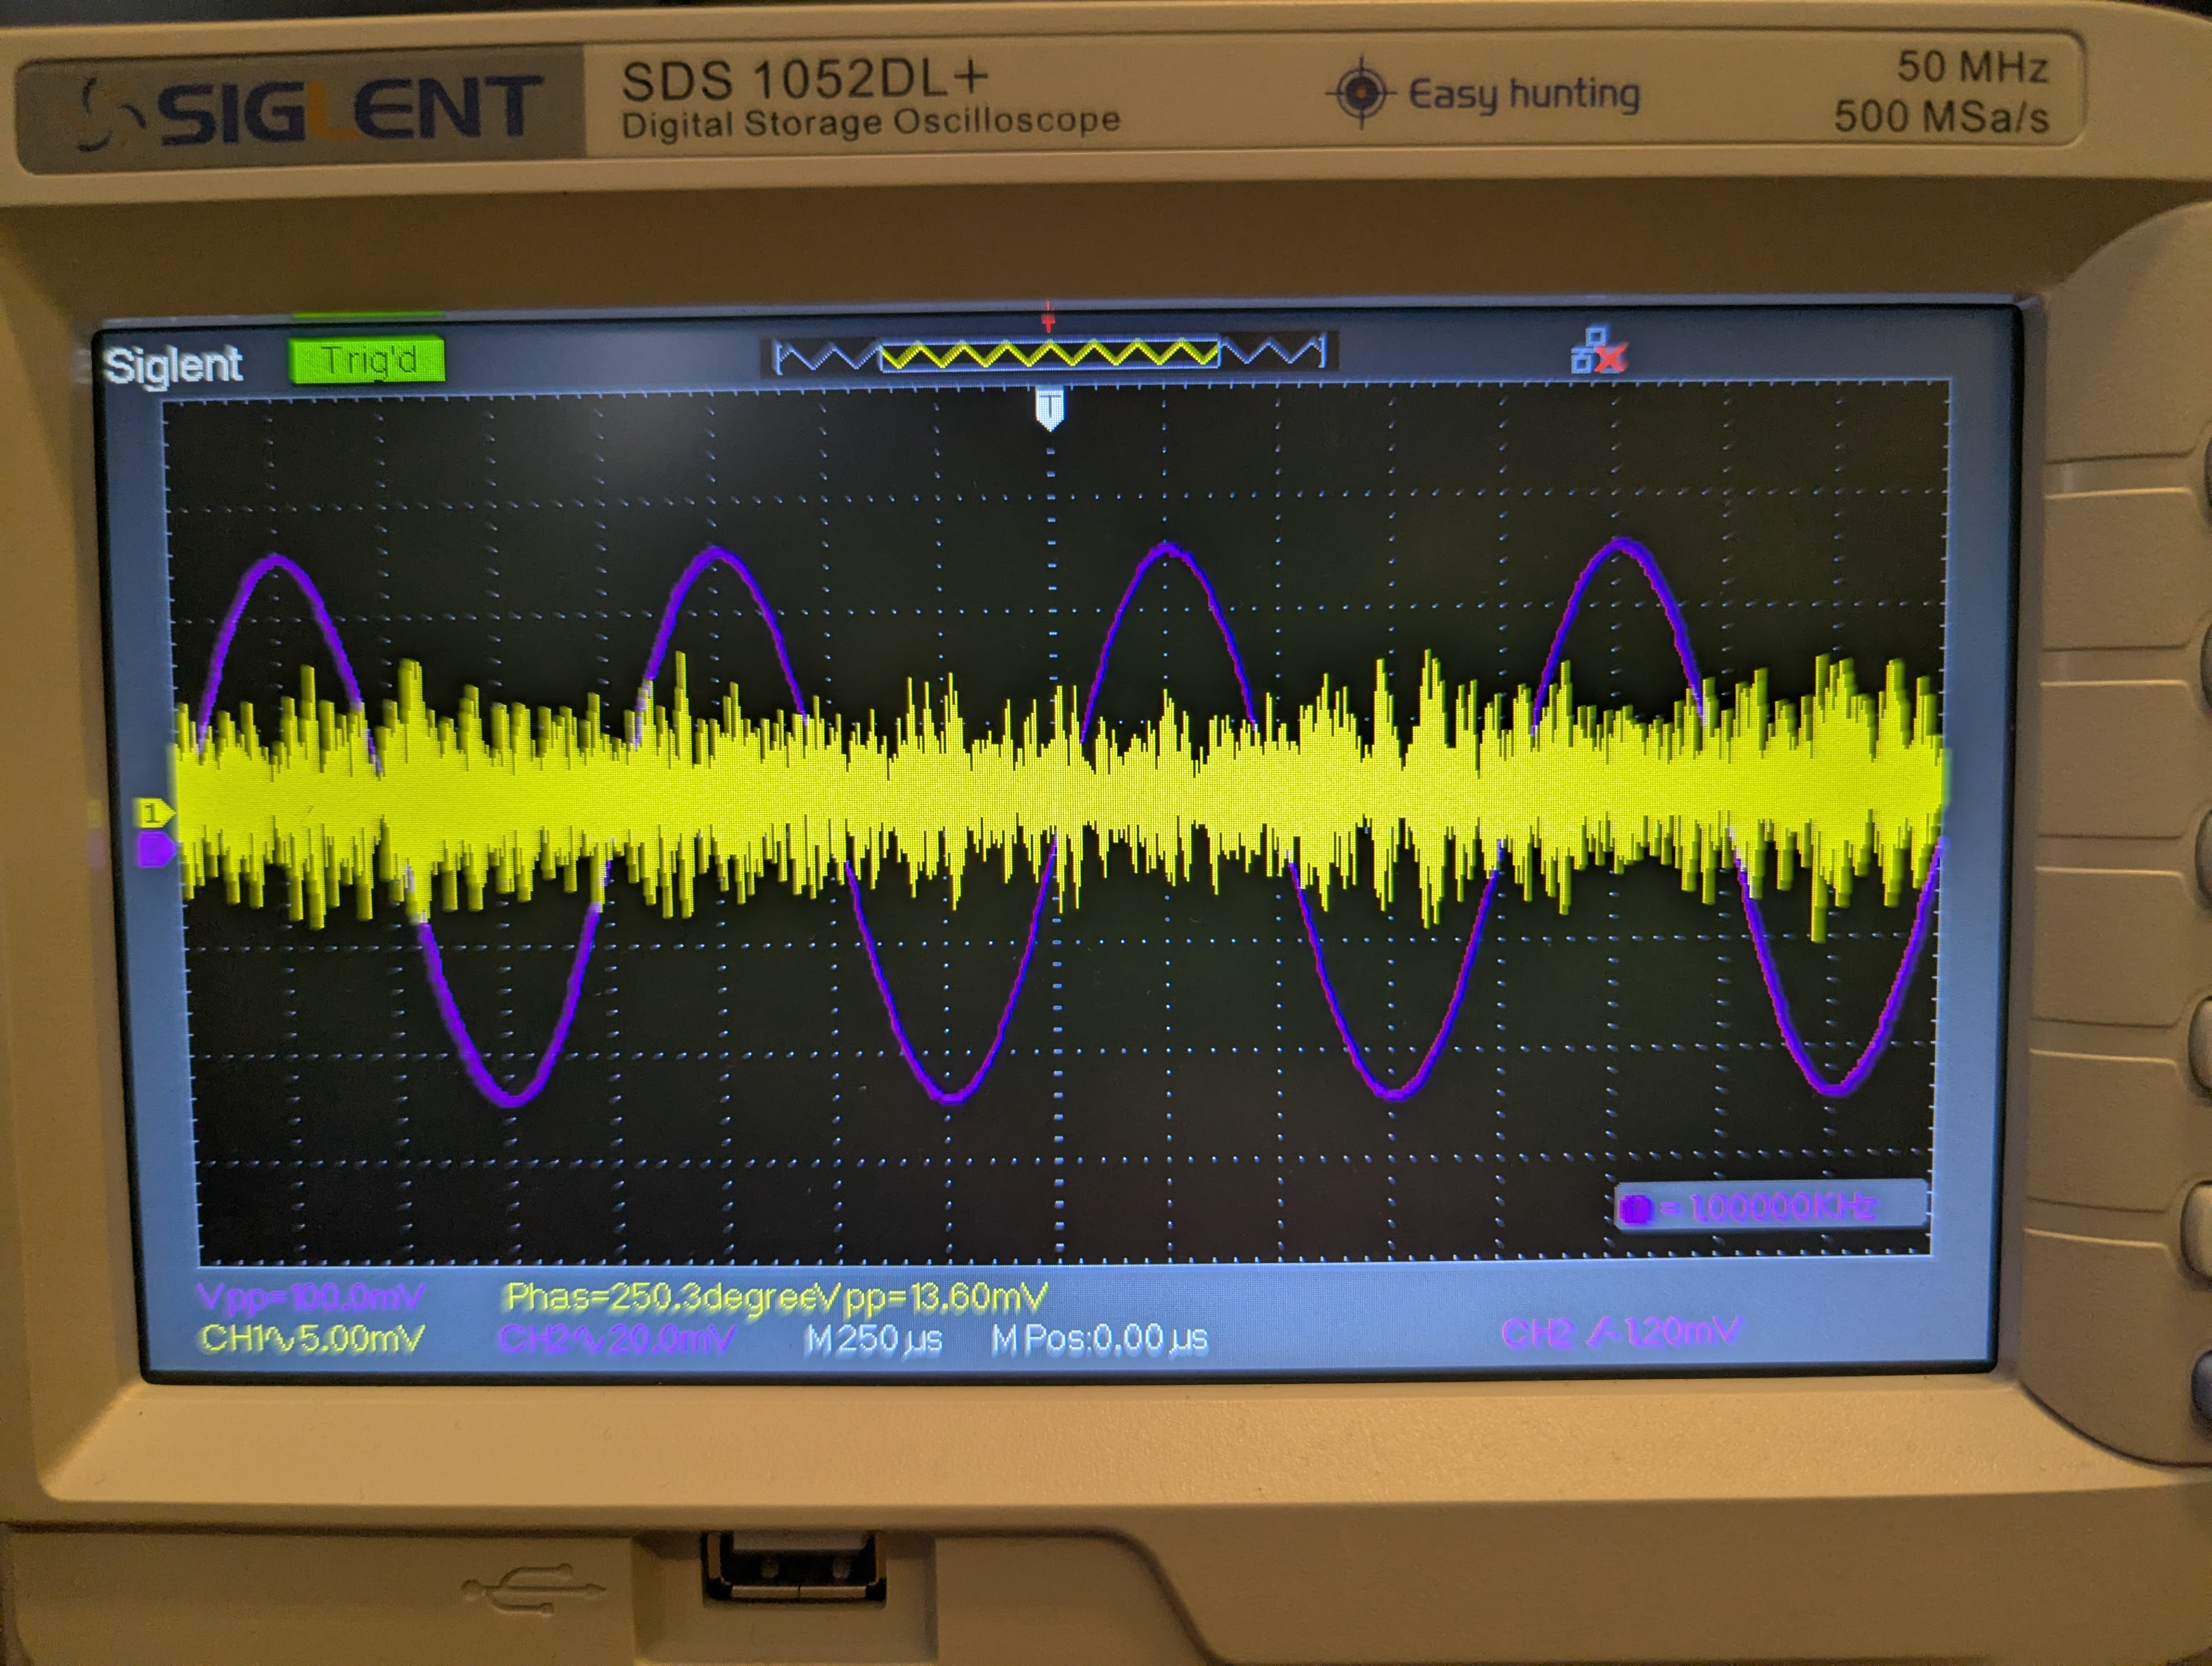
\includegraphics[width=\linewidth]{int_sine_no.jpg} 
    \end{subfigure}
    \begin{subfigure}[b]{0.32\linewidth}
        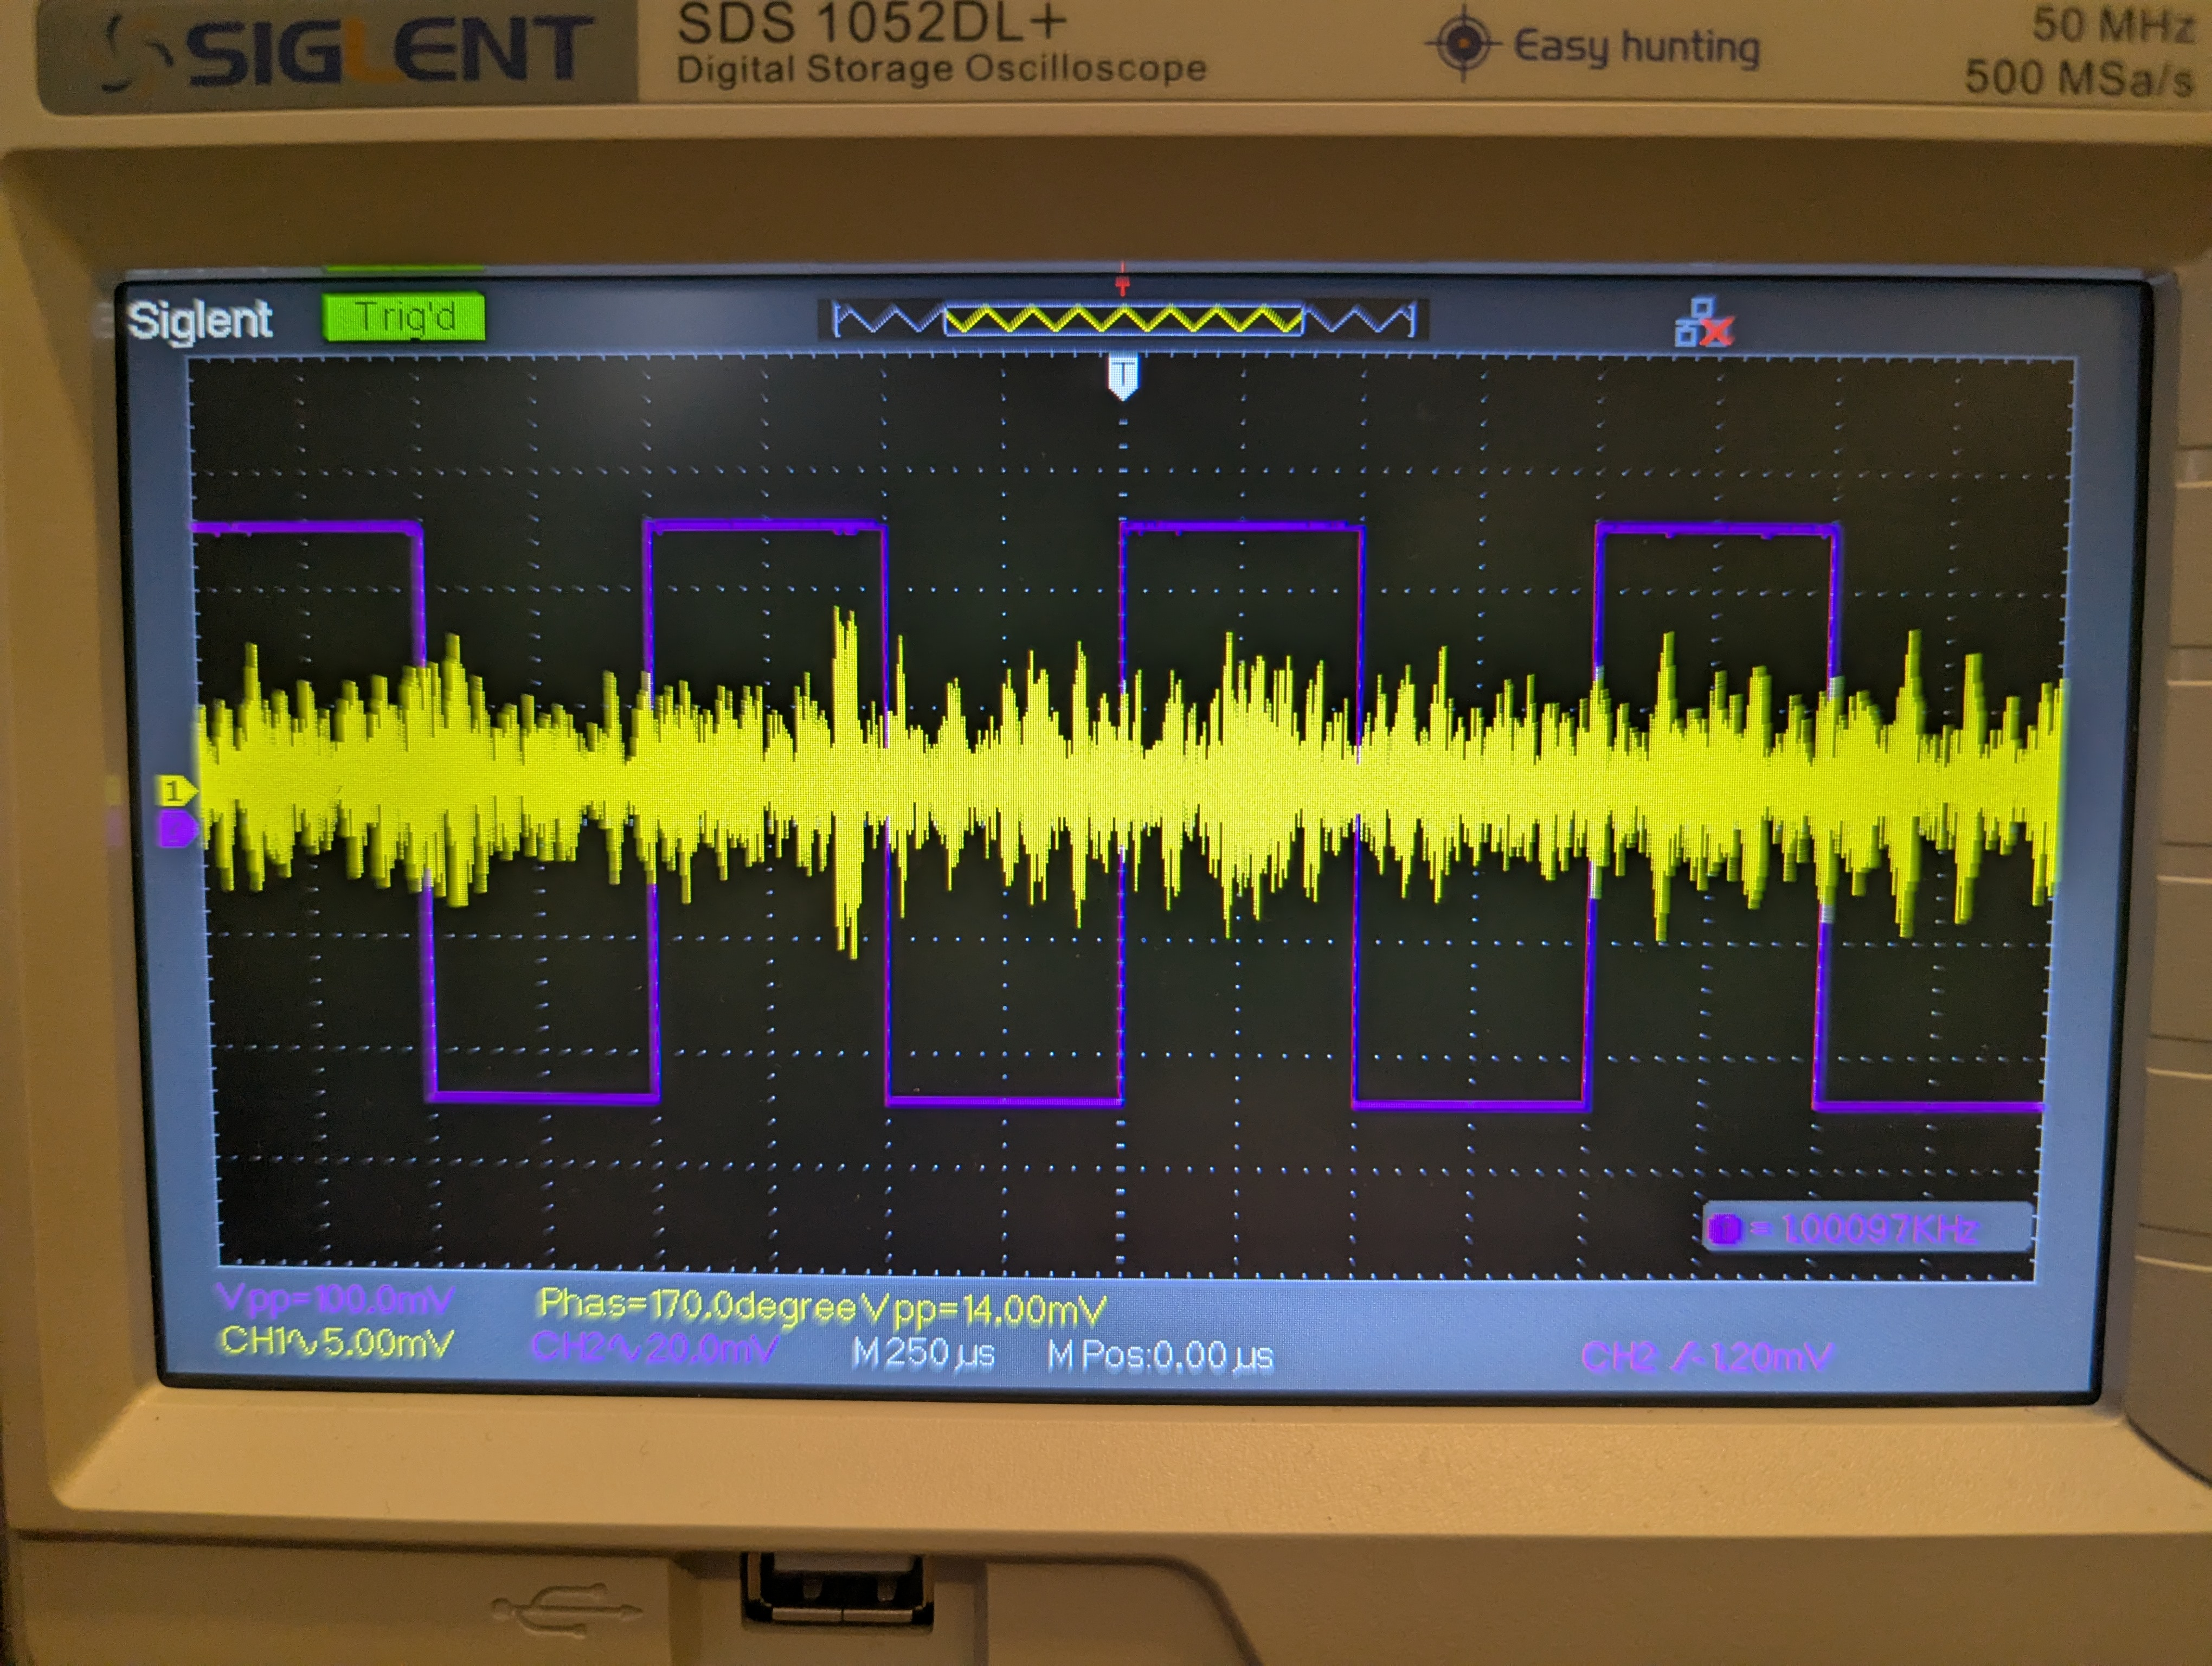
\includegraphics[width=\linewidth]{int_square_no.jpg} 
    \end{subfigure}
    \begin{subfigure}[b]{0.32\linewidth}
        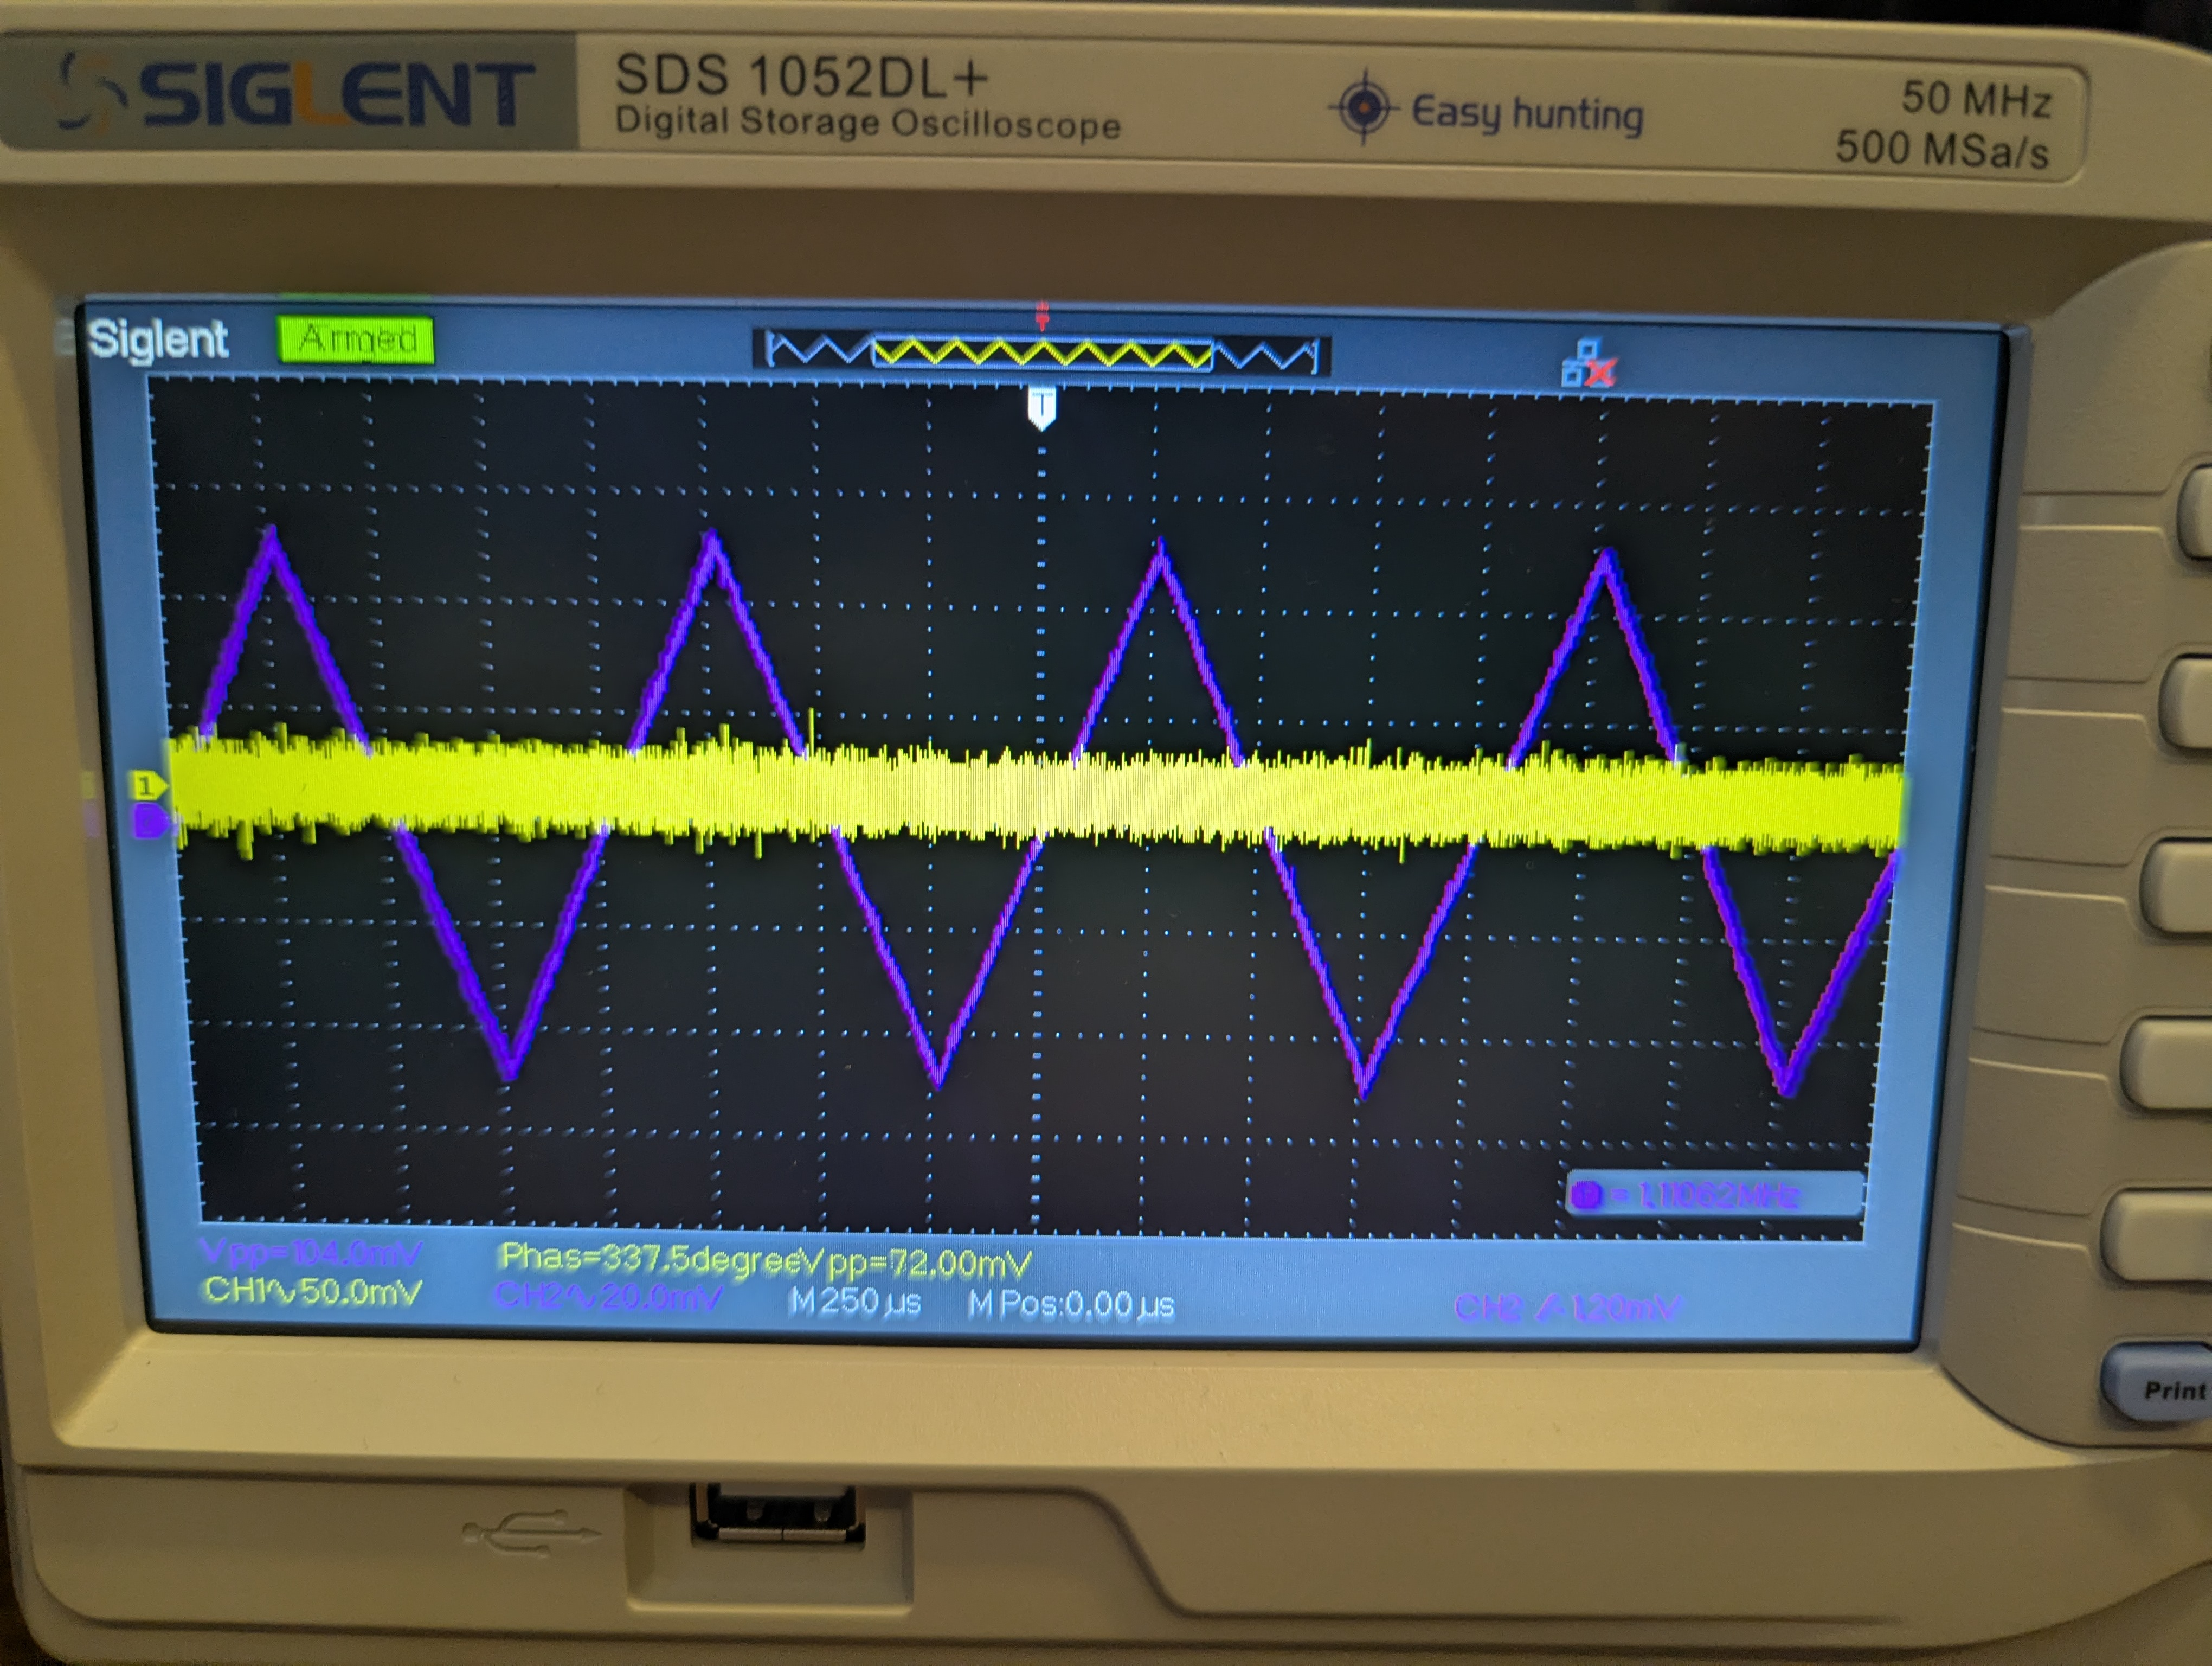
\includegraphics[width=\linewidth]{int_triangle_no.jpg} 
    \end{subfigure}
    \caption{Integrator output waveforms for sine, square, and triangle inputs \textbf{without} the feedback resistor \(R_p\), showing drift and saturation.}
    \label{fig:integrator_no}
\end{figure}




\section{Conclusion}
This series of experiments successfully demonstrated the fundamental principles of several basic operational amplifier circuits. The measured gain of the inverting amplifier closely matched the theoretical value. The functions of the adder, voltage follower, differentiator, and integrator circuits were verified, and their outputs for various input signals were observed to be in line with theoretical predictions. The roles of supplementary components for stability and noise reduction, such as the parallel capacitor in the differentiator and the feedback resistor in the integrator, were also practically demonstrated and understood. The discrepancies and practical issues encountered, such as component failures and saturation, highlighted the differences between ideal models and real-world circuit behavior.

\end{document}